\documentclass{article}
\usepackage[T1]{fontenc}
\usepackage{amsmath,amssymb,mathtools,booktabs,multirow,colortbl,url,float}
\usepackage[lined,boxed,commentsnumbered]{algorithm2e}
\usepackage{algpseudocode}
\algnewcommand{\Initialize}[1]{%
  \State \textbf{Initialize:}
  \Statefx \hspace*{\algorithmicindent}\parbox[t]{.8\linewidth}{\raggedright #1}
}


\DeclareMathOperator{\sign}{sign}
\DeclarePairedDelimiter\norm{\lVert}{\rVert}%
\DeclarePairedDelimiter\abso{\lvert}{\rvert}%
\DeclareMathOperator*{\argmin}{arg\,min}
\DeclareMathOperator*{\argmax}{arg\,max}

\newcommand\myeq{\stackrel{\mathclap{\normalfont\mbox{def}}}{=}}

\newtheorem{definition}{Definition}
\newtheorem{theorem}{Theorem}
\newtheorem{example}{Example}


\usepackage[most]{tcolorbox}
\newtcolorbox{mymathbox}[1][]{colback=white, sharp corners, #1}
\colorlet{colexam}{red!60!black}
\newtcolorbox{testexample}[1][]{
    empty,
    title={Example: #1},
    % attach boxed title to top left,
    minipage boxed title,
    boxed title style={empty,size=minimal,toprule=0pt,top=4pt,left=3mm,overlay={}},
    coltitle=colexam,
    fonttitle=\bfseries,
    before=\par\medskip\noindent,parbox=false,boxsep=0pt,left=3mm,right=0mm,top=2pt,breakable,pad at break=0mm,
    before upper=\csname @totalleftmargin\endcsname0pt,
    %
    overlay unbroken={\draw[colexam,line width=.5pt] ([xshift=-1.2pt]title.north west) -- ([xshift=-0pt]frame.south west); },
    %
    overlay first={\draw[colexam,line width=.5pt] ([xshift=-0pt]title.north west) -- ([xshift=-0pt]frame.south west); },
    %
    overlay middle={\draw[colexam,line width=.5pt] ([xshift=-0pt]frame.north west) -- ([xshift=-0pt]frame.south west); },
    %
    overlay last={\draw[colexam,line width=.5pt] ([xshift=-0pt]frame.north west) -- ([xshift=-0pt]frame.south west); }
    }
\colorlet{colspec}{blue!60!black}
\newtcolorbox{spexample}[1][]{
    empty,
    title={#1},
    % attach boxed title to top left,
    minipage boxed title,
    boxed title style={empty,size=minimal,toprule=0pt,top=4pt,left=3mm,overlay={}},
    coltitle=colspec,
    fonttitle=\bfseries,
    before=\par\medskip\noindent,parbox=false,boxsep=0pt,left=3mm,right=0mm,top=2pt,breakable,pad at break=0mm,
    before upper=\csname @totalleftmargin\endcsname0pt,
    %
    overlay unbroken={\draw[colspec,line width=.5pt] ([xshift=-1.2pt]title.north west) -- ([xshift=-0pt]frame.south west); },
    %
    overlay first={\draw[colspec,line width=.5pt] ([xshift=-0pt]title.north west) -- ([xshift=-0pt]frame.south west); },
    %
    overlay middle={\draw[colspec,line width=.5pt] ([xshift=-0pt]frame.north west) -- ([xshift=-0pt]frame.south west); },
    %
    overlay last={\draw[colspec,line width=.5pt] ([xshift=-0pt]frame.north west) -- ([xshift=-0pt]frame.south west); }
    }

\usepackage{bm}
\usepackage[a4paper, total={6in, 8in}]{geometry}
\usepackage{enumerate}

\usepackage{concmath}
\pdfpkmode{supre} \pdfpkresolution=2400

\def\oldstylenums#1{%
\begingroup
\spaceskip\fontdimen\tw@\font
\usefont{OML}{ccm}{\f@series}{it}%
\mathgroup\symletters #1%
\endgroup}

\DeclareMathOperator{\di}{d\!}




\title{\textbf{Advanced Machine  Learning}\\Informal syllabus}
\author{Erik Koene}
\date{November 2018}

\begin{document}

\maketitle
% See for background material e.g., Bishop: Pattern Recognition And Machine Learning (2006).

\setcounter{section}{-2}
\section{The historical setting of statistical learning theory}
This section, starting of at minus 1, is mostly based on \textsc{Vladimir Vapnik}'s \textit{The Nature of Statistical Learning -- for Engineering and Information Science} (1995) and more thorough \textit{Statistical Learning Theory} (1998). This background information is interesting to set up the topic.

\subsection{Parametric inference, 1920s--1960s}
By the 1920s, descriptive statistics was mostly complete: statistical laws (distribution functions) were found to describe various events of reality well. The next topic was that of \textbf{statistical inference}: when given a collection of empirical data origination from some functional dependency, infer this dependency. The two main approaches to this issue were the following:
\begin{enumerate}
    \item The particular (parametric) inference, when the investigator knows the problem to be analyzed well enough to assume the statistical law and target function: the problem then reduces to finding the optimal parameters using the maximum likelihood method.
    \item The general inference, when one does not have reliable a priori information about the statistical law underlying the problem or about the function that one would like to approximate.
\end{enumerate}
The first approach (parametric inference) to inductive inference had its ``golden age'' between the 1930s and 1960s, in the time before computers, when simple methods were the only realizable option. The philosophy of the parametric approach assumed that:
\begin{enumerate}
    \item \textit{A set of functions, linear and minimal in their parameters, contains a good approximation to the desired function},
    \item \textit{The statistical law underlying the stochastic component of most real-life problems is the normal law},
    \item \textit{The maximum likelihood method is a good tool for estimating the parameters}.
\end{enumerate}
However the wide avialability of computers in the 60s showed that all three beliefs had shortcomings:
\begin{enumerate}
    \item In realistic multidimensional problems with dozens or even hundreds of variables, the belief that one can define a reasonably small set of functions that contains a good approximation to a desired one is wrong, also through the `curse of dimensionality' (\textsc{R. Bellman}).
    \item Additionally, \textsc{Tukey} found that real-life data often differs from classical statistical distribution functions, and one must take this into account to construct effective algorithms.
    \item \textsc{James} and \textsc{Stein} showed that even for simple problems of density estimation, such as finding the mean of a $n>2$-dimensional Gaussian with unit covariance, the maximum likelihood method is not the best one. The estimator they suggest is uniformly better than the maximum likelihood estimator!
\end{enumerate}
Thus, the beliefs upon which parametric inductive inference was based turn out to be inappropriate for many real-life problems, opening the door for other methods of statistical inference.

\subsection{Inductive inference, 1970s--2000s}
\textsc{Rosenblatt} introduced a computer program in 1958, based on a neurophysiological learning model called the Perceptron, which happened to generalize well to classification problems. Consequently, \textsc{Novikov} proved a series of theorems about the Perceptron, particularly that it will converge to a solution in a finite number of iterations. (As a side-note, \textsc{Minsky \& Papert} released a book called `Perceptrons' in 1969 that proved that these neurons couldn't solve some very simple problems. This negative outlook led to a decline in interest in AI called the `AI winter' -- computers can't do \textit{logic}. However, from the ashes came `machine learning', which tries to do much smaller, humbler, tasks and side-step questions of logic, and is based on \textbf{statistics and optimization}.) Thus arose the question \textit{how, and under which constraints, can we generalize algorithms that are agnostic to the underlying probability density function}? And so, \textbf{statistical learning theory} is born!

The fundamental answer in statistical learning theory was found through \textit{empirical risk minimization} (ERM): to generalize well to new data, we must minimize a specific \textit{loss function} for our training data. The ERM principle yields the maximum likelihood method when we choose a logarithmic loss, but generalizes to many more varied decision rules! Machine learning is now similar to an optimization procedure, but requires you to choose the right optimization strategy!

While algorithmic advances went slow (it took until 1986 before the back-propagation technique for neural networks was discovered by \textsc{LeCun}), much more progress was attained in theoretical advances. \textsc{Vapnik} and \textsc{Chervonenkis} developed the ERM theory to obtain minimal generalization error with only limited data. A particular insight was that we can simplify things when we want to predict values only in a \textit{limited} range. The old parametric paradigm uses a two-stage procedure that is called \textbf{generative modeling}: at the first (induction) stage we estimate the probability density function, at the second (deduction) stage we use this function to compute values at new points of interest. The first step thus solves a problem that is more general than the one required, for it estimates the \textit{entire} unknown function for \textit{all} points on the domain. This is expensive and difficult to do well. When we only want to estimate the values of a function at a few points of interest, with a restricted amount of information, it is possible to estimate the unknown function in one immediate (transduction) step: \textbf{discriminative modeling}.

\subsection{Neural networks, 2010s--present}
Then, with the rise of `big data' and very powerful computers, multilayer perceptrons (or `neural networks') started to outperform other methods developed with the ERM principle, and win many machine learning competitions! However, the methods require a lot of `fiddling the knobs' to obtain good results, and the statistical community is playing catch-up to understand how to make the neural nets learn optimally and stably.

\newpage

\section{Prerequisites (informal introduction)}
\subsection{Probability}
We define $\mathbb{P}(A)$ as the probability of event $A$ to be measured from the set of \textit{all} possible outcomes, mapping to a number within $[0,1]$. We define $\mathbb{P}(A\cap B)=\mathbb{P}(A,B)$ as the probability of the set intersection (the common elements in $A$ and $B$). Notably, for every event $A$ there is the complement of $A^c$ for which we have:
\begin{align}
    \mathbb{P}(A\cap A^c)=\mathbb{P}(\varnothing)&=0,&
    \mathbb{P}(A) + \mathbb{P}(A^c)&=1.
\end{align}
When probabilities are \textit{\textbf{indepedent}} (the outcome of one event doesn't influence the likelihood of another event; they happen in arbitrary order), it is implied that $\mathbb{P}(A,B)=\mathbb{P}(A)\mathbb{P}(B)$.
\begin{testexample}[Throwing dice, part 1]
    We'll roll two dice, and consider event $A$ to represent that the first throw is $i\in\{1,2,3,4\}$ and the second throw is $j\in\{4,5,6\}$. Event $B$ is an outcome where the two dice sum to the number 7. The valid \textit{sample space} of $A$ and $B$ is here tabulated in {\color{gray} gray}:
    
\begin{center}
\hfill
    \begin{tabular}{@{}ll|llllll}
\toprule
A & & \multicolumn{6}{c}{$j$} \\ 
 & $(\cdot,\cdot)$ & 1 & 2 & 3 & \cellcolor{gray!10}4 & \cellcolor{gray!10}5 & \cellcolor{gray!10}6 \\ \hline
\multirow{6}{*}{$i$} & \cellcolor{gray!10}1 & (1,1) & (1,2) & (1,3) & \cellcolor{gray!20}(1,4) & \cellcolor{gray!20}(1,5) & \cellcolor{gray!20}(1,6) \\
 & \cellcolor{gray!10}2 & (2,1) & (2,2) & (2,3) & \cellcolor{gray!20}(2,4) & \cellcolor{gray!20}(2,5) & \cellcolor{gray!20}(2,6) \\
 & \cellcolor{gray!10}3 & (3,1) & (3,2) & (3,3) & \cellcolor{gray!20}(3,4) & \cellcolor{gray!20}(3,5) & \cellcolor{gray!20}(3,6) \\
 & \cellcolor{gray!10}4 & (4,1) & (4,2) & (4,3) & \cellcolor{gray!20}(4,4) & \cellcolor{gray!20}(4,5) & \cellcolor{gray!20}(4,6) \\
 & 5                    & (5,1) & (5,2) & (5,3) & (5,4) & (5,5) & (5,6) \\
 & 6                    & (6,1) & (6,2) & (6,3) & (6,4) & (6,5) & (6,6) \\ \bottomrule
\end{tabular}
\hfill
    \begin{tabular}{@{}ll|llllll}
\toprule
B & & \multicolumn{6}{c}{$j$} \\ 
 & + & 1 & 2 & 3 & 4 & 5 & 6 \\ \hline
\multirow{6}{*}{$i$} & 1 & 2 & 3 & 4 & 5 & 6 & \cellcolor{gray!20}7 \\
 & 2 & 3 & 4 & 5 & 6 & \cellcolor{gray!20}7 & 8 \\
 & 3 & 4 & 5 & 6 & \cellcolor{gray!20}7 & 8 & 9 \\
 & 4 & 5 & 6 & \cellcolor{gray!20}7 & 8 & 9 & 10 \\
 & 5 & 6 & \cellcolor{gray!20}7 & 8 & 9 & 10 & 11 \\
 & 6 & \cellcolor{gray!20}7 & 8 & 9 & 10 & 11 & 12 \\ \bottomrule
\end{tabular}
\hfill
\end{center}
    Throws $i,j$ are independent, such that $\mathbb{P}(i,j)=\mathbb{P}(i)\mathbb{P}(j)=\frac{1}{6}\frac{1}{6}=\frac{1}{36}$. The probabilities are then given by summing over the number of elements in the set (the cardinalities $|A|$ and $|B|$):
    \begin{align*}
        \mathbb{P}(A)&=|A|\frac{1}{36}=\frac{(4\cdot 3)}{36}=\frac{1}{3},& \mathbb{P}(A^c)&=1-\mathbb{P}(A)=\frac{2}{3},&  \mathbb{P}(B)&=|B|\frac{1}{6}=\frac{6}{36}=\frac{1}{6}.
    \end{align*}
    If we want the intersection of $A$ and $B$, we are left with three valid outcomes:
    \begin{equation*}
        A\cap B = \{ \{1,6\},\{2, 5\},\{3,4\} \},
    \end{equation*}
    such that we can write:
    \begin{equation*}
        \mathbb{P}(A\cap B)=\mathbb{P}(A,B)=\frac{3}{36}=\frac{1}{12} \quad \Bigg( \neq \mathbb{P}(A)\mathbb{P}(B) \Bigg).
    \end{equation*}
\end{testexample}
{\flushleft Formally}, for events $A$ and $B$ from the set of all possible outcomes $\Omega$, we have:
\begin{mymathbox}[ams align, title={Probability of events $A,B\in\Omega$}, colframe=blue!30!black, center title]
	\mathbb{P}(A) & \geq 0, \quad \forall A\in\Omega,\\
	\mathbb{P}(\Omega) & = 1,\\
	A,B\text{\ independent\ }\Longrightarrow\mathbb{P}(A\cap B) = \mathbb{P}(A,B) & = \mathbb{P}(A)\mathbb{P}(B), \quad \forall (A,B)\in\Omega
\end{mymathbox}

\subsection{Conditional probability}
We define $\mathbb{P}(A|B)\equiv\mathbb{P}(A,B)/\mathbb{P}(B)$ as the conditional probability of event $A$, given that $B$ \textit{has already occurred}. It is to be read as `the probability of outcome $A$, given outcome $B$'. Everything behind the bar $|$ is the condition on $A$. It is one of the most fundamental concepts of statistics, but also a bit slippery and requires great care in interpretation! Particularly that $\mathbb{P}(A|B)\neq\mathbb{P}(B|A)$.
\begin{testexample}[Throwing dice, part 2]
    Continuing from the previous example, say that we are interested in the probability of $\mathbb{P}(B|A)$, thus that our dice sum up to $7$, but we know that the throw ended up in the valid sample space of $A$. This means that our sample space is much reduced, it is only that region where $A$ is valid:
    \begin{center}
    \begin{tabular}{@{}ll|llllll}
\toprule
$B|A$ & & \multicolumn{3}{c}{$j$} \\ 
 & + & 4 & 5 & 6 \\ \hline
\multirow{4}{*}{$i$} & 1 & 5 & 6 & \cellcolor{gray!20}7 \\
  & 2 & 6 & \cellcolor{gray!20}7 & 8 \\
  & 3 & \cellcolor{gray!20}7 & 8 & 9 \\
  & 4 & 8 & 9 & 10 \\ \bottomrule
\end{tabular}
\end{center}
The valid sample space of $B$, given $A$, is now reduced, and $1/4$-th of its possible outcomes now generate event $B$! We can find the same result in a general way using our previously found probabilities and the conditional probability rule:
\begin{equation}
    \mathbb{P}(B|A)=\frac{\mathbb{P}(A,B)}{\mathbb{P}(A)}=\frac{\dfrac{1}{12} }{\dfrac{1}{3} }=\frac{3}{12}=\frac{1}{4}.
\end{equation}
It is thus the \textit{reduction of the sample space} that the probability changes -- knowing that outcome $A$ applies makes it more likely that our dice sum to 7!
\end{testexample}
{\flushleft We} can rearrange the rule of conditional probability in three ways, which are all informative:
\begin{align}
    \mathbb{P}(A|B)&=\frac{\mathbb{P}(A,B)}{\mathbb{P}(B)},& \mathbb{P}(B)&=\frac{\mathbb{P}(A,B)}{\mathbb{P}(A|B)},& \mathbb{P}(A,B)=\mathbb{P}(A|B)\mathbb{P}(B).
\end{align}
Note that for \textbf{\textit{independent}} $A$ and $B$, for which $\mathbb{P}(A,B)=\mathbb{P}(A)\mathbb{P}(B)$ you easily obtain:
\begin{align}
    \mathbb{P}(A|B)&=\frac{\mathbb{P}(A)\mathbb{P}(B)}{\mathbb{P}(B)}=\mathbb{P}(A).
\end{align}
Knowing about state $B$ thus gives no information about state $A$.
For example, you throw a die and flip a coin, and $A$ tests the number of the die while $B$ tests the side of the coin. There is then no information gained about state $B$ when we learn about $A$, or vice versa.

\begin{mymathbox}[ams align, title={Conditional probability of $(A,B)\in\Omega$ (definition)}, colframe=blue!30!black, center title]
	\mathbb{P}(A|B) & \equiv \frac{\mathbb{P}(A\cap B)}{\mathbb{P}(B)}, \quad \forall (A,B)\in\Omega.
\end{mymathbox}

\subsection{Marginal probability}
Given a set of joint probabilities $(A,B_1),(A,B_2),\dots$ with events $B_n$ a disjoint partition (no element occurs in more than one set), we find the total chance $A$ by summing over all sub-sets:
\begin{equation}
    \mathbb{P}(A) = \sum_n \mathbb{P}(A,B_n).
\end{equation}
As seen in the previous section, this may also be written in terms of conditional probabilities:
\begin{equation}
    \mathbb{P}(A) = \sum_n \mathbb{P}(A|B_n)\mathbb{P}(B_n).
\end{equation}
It is thus a \textit{weighted average} of the conditional probabilities.
\begin{testexample}[Buying light bulbs]
    Assume that factory $X$ produces 60\% of all light bulbs, which work over 5000 hours in 99\% of the cases, while factory $Y$ produces 40\% of all light bulbs, which work over 5000 hours in 95\% of the cases. The chance that a purchased light-bulb works at least 5000 hours is then:
    \begin{equation}
        \mathbb{P}(\text{works}) = \mathbb{P}(\text{works}|F_X)\mathbb{P}(F_X) + \mathbb{P}(\text{works}|F_Y)\mathbb{P}(F_Y) = \frac{99}{100}\frac{60}{100} + \frac{95}{100}\frac{40}{100} = 97.4\%.
    \end{equation}
    Indeed, the marginal probability is a weighted average of the conditional probabilities.
\end{testexample}
\begin{testexample}[Getting hit by cars]
    Assume that we know the conditional probability of being hit by a car $H$ for three traffic light colors $L$, as well as the probability of observing a particular traffic light state:
    \begin{center}
        \begin{tabular}{@{}lr|lll@{}}
        \toprule
        & & \multicolumn{3}{c}{$L$} \\ 
        &  & Red & Yellow & Green \\ \hline
        \multirow{2}{*}{$\mathbb{P}(H|L)\quad\quad H$} & Not hit & 0.99 & 0.9 & 0.2 \\
        & Hit & 0.01 & 0.1 & 0.8 \\ \cline{1-5}
        $\mathbb{P}(L)$& & 0.2 & 0.1 & 0.7 \\
        \bottomrule
        \end{tabular}
    \end{center}
    We can now compute the joint probability, $\mathbb{P}(H_p,L_n)=\mathbb{P}(H_p|L_n)\mathbb{P}(L_n)$:
    \begin{center}
        \begin{tabular}{lr|lll|l}
        \toprule
         & & \multicolumn{3}{c|}{$L$} & \cellcolor{gray!20} \\ 
        &$\mathbb{P}(H_p,L_n)$  & Red & Yellow & Green & \cellcolor{gray!20}$\sum_n \mathbb{P}(H_p,L_n)=\mathbb{P}(H_p)$ \\ \cline{2-6}\omit \vrule height.4pt\textcolor[rgb]{0,0,0}{\leaders\vrule\hfil}\vrule \cr
        \multirow{2}{*}{$H$} & Not hit & 0.198 & 0.09 & 0.14 & \cellcolor{gray!20}0.428 \\
        & Hit & 0.002 & 0.01 & 0.56 & \cellcolor{gray!20}0.572 \\ \cline{2-6}\omit \vrule height.4pt\textcolor[rgb]{0,0,0}{\leaders\vrule\hfil}\vrule \cr
        \cellcolor{gray!20}& \cellcolor{gray!20}$\sum_p\mathbb{P}(H_p,L_n)=\mathbb{P}(L_n)$ & \cellcolor{gray!20}0.2 & \cellcolor{gray!20}0.1 & \cellcolor{gray!20}0.7 & \cellcolor{gray!20}1 \\ \bottomrule
        \end{tabular}
    \end{center}
    The bottom row and right column (the \textit{margins} of the table!) now provide the marginal chances: $\mathbb{P}(\text{Red})=0.2$, $\mathbb{P}(\text{Not hit})=0.428$, etc., by summing over the corresponding row or column. They provide the sum of the conditional outcomes, weighed by the chance of each condition happening.
\end{testexample}


\begin{mymathbox}[ams align, title={Law of total probability, when $\Omega$ is split wholly into $n$ portions}, colframe=blue!30!black, center title]
	\mathbb{P}(A) & = \sum_n\mathbb{P}(A,B_n) = \sum_n \mathbb{P}(A|B_n)\mathbb{P}(B_n), \quad \forall A\in\Omega\text{, and disjoint }\bigcup_n B_n=\Omega.
\end{mymathbox}

\subsection{Bayes' rule}
We may realize that intersections are identical regardless of their order ($A\cap B=B\cap A$), and find the following identical conditional probabilities:
\begin{align}
    \mathbb{P}(A,B) &=\mathbb{P}(B,A), \\
    \mathbb{P}(A|B)\mathbb{P}(B) &= \mathbb{P}(B|A)\mathbb{P}(A).
\end{align}
Re-writing this identity provides Bayes' rule, with which we can invert conditional probabilities:
\begin{equation}
    \mathbb{P}(A|B) = \frac{\mathbb{P}(B|A)\mathbb{P}(A)}{\mathbb{P}(B)}.
\end{equation}
\begin{testexample}[Drug-testing]
    A drug-test gives 99\% true positives on drug-users and 98\% true negatives on non-drug-users. Suppose that 0.5\% of the population uses the drug. Then we compute the probability that a positive test really is due to a drug-user:
    \begin{equation}
        \mathbb{P}(\text{drug-user}|+) = \frac{\mathbb{P}(+|\text{drug-user})\mathbb{P}(\text{drug-user})}{ \mathbb{P}(+) } = \frac{0.99\cdot0.005}{\mathbb{P}(+)}
    \end{equation}
    We can compute $\mathbb{P}(+)$, i.e., the chance of finding a positive result regardless of whether the user actually took drugs, by taking the sum of the true and false positives. In other words, we \textit{marginalize} over the state of the users!
    \begin{align}
        \mathbb{P}(\text{drug-user}|+)& = \frac{0.99\cdot0.005}{\mathbb{P}(+|\text{drug-user})\mathbb{P}(\text{user})+\mathbb{P}(+|\text{non-drug-user})\mathbb{P}(\text{non-drug-user})},\\
        &=\frac{0.99\cdot0.005}{0.99\cdot0.005+0.02\cdot 0.995},\\
        &=20\%.
    \end{align}
    The test thus performs surprisingly poorly on the global population: only in 20\% of the cases will a positive test result indicate that the test subject truly used the drug! But realize that for a 1000 subjects, we expect 5 users and 995 non-users. From those 995 users, $0.02\cdot995\approx 20$ false positives will occur, while we will catch all five true users, $0.99\cdot5\approx 5$. Out of 25 positive results, only 5 are thus genuine!
\end{testexample}
{\flushleft We} can thus write two versions of Bayes' rule, the second one where we marginalize in the denominator over the quantity of interest.
\begin{mymathbox}[ams align, title={Bayes' rule}, colframe=blue!30!black, center title]
	\mathbb{P}(B|A) &= \frac{\mathbb{P}(A|B)\mathbb{P}(B)}{\mathbb{P}(A)}, \quad &\forall& (A,B)\in\Omega,\label{eq:bayes1} \\
	\mathbb{P}(B_j|A) &= \frac{\mathbb{P}(A|B_j)\mathbb{P}(B_j)}{\sum_n \mathbb{P}(A|B_n)\mathbb{P}(B_n)}\quad &\forall& A\in\Omega\text{, and disjoint }\bigcup_n B_n=\Omega.\label{eq:bayes2}
\end{mymathbox}

\subsection{Indicator function}
We define an indicator function $\mathbb{I}_{X=x}$, which is 1 when the statement $X=x$ is true, and 0 otherwise.
\begin{testexample}[Bayesian dice experiment]
    Two dice are thrown that sum to 9. What is the posterior distribution of the dice rolls? In other words, what dice combinations are likely, given that we know that they sum to 9?
    
    We define event $A$ for two dice $i,j$ to sum to $9$. We thus have the following Bayesian' rule:
    \begin{equation}
        \mathbb{P}(i,j|A) = \frac{ \mathbb{P}(A|i,j)\mathbb{P}(i,j)}{\mathbb{P}(A)}.
    \end{equation}
    The prior is the uniform distribution we have seen before, $\mathbb{P}(i,j)=\mathbb{P}(i)\mathbb{P}(j)$. The likelihood is expressed with an indicator function $\mathbb{P}(A|i,j)=\mathbb{I}_{i+j=9}$: after the two dice are rolled and known, they either sum to 9 or not! These two results are expressed in tabular form as:
    \begin{center}
    \hfill
\begin{tabular}{@{}lr|llllll}
\toprule
 & & \multicolumn{6}{c}{$j$} \\ 
 &$\mathbb{P}(i,j)$ & 1 & 2 & 3 & 4 & 5 & 6 \\ \hline
\multirow{6}{*}{$i$} & 1 & $^{1\!}/_{\! 36}$ & $^{1\!}/_{\! 36}$ & $^{1\!}/_{\! 36}$ & $^{1\!}/_{\! 36}$ & $^{1\!}/_{\! 36}$ & $^{1\!}/_{\! 36}$ \\
 & 2 & $^{1\!}/_{\! 36}$ & $^{1\!}/_{\! 36}$ & $^{1\!}/_{\! 36}$ & $^{1\!}/_{\! 36}$ & $^{1\!}/_{\! 36}$ & $^{1\!}/_{\! 36}$ \\
 & 3 & $^{1\!}/_{\! 36}$ & $^{1\!}/_{\! 36}$ & $^{1\!}/_{\! 36}$ & $^{1\!}/_{\! 36}$ & $^{1\!}/_{\! 36}$ & $^{1\!}/_{\! 36}$ \\
 & 4 & $^{1\!}/_{\! 36}$ & $^{1\!}/_{\! 36}$ & $^{1\!}/_{\! 36}$ & $^{1\!}/_{\! 36}$ & $^{1\!}/_{\! 36}$ & $^{1\!}/_{\! 36}$ \\
 & 5 & $^{1\!}/_{\! 36}$ & $^{1\!}/_{\! 36}$ & $^{1\!}/_{\! 36}$ & $^{1\!}/_{\! 36}$ & $^{1\!}/_{\! 36}$ & $^{1\!}/_{\! 36}$ \\
 & 6 & $^{1\!}/_{\! 36}$ & $^{1\!}/_{\! 36}$ & $^{1\!}/_{\! 36}$ & $^{1\!}/_{\! 36}$ & $^{1\!}/_{\! 36}$ & $^{1\!}/_{\! 36}$ \\ \bottomrule
\end{tabular}
\hfill
\begin{tabular}{@{}lr|llllll}
\toprule
 & & \multicolumn{6}{c}{$j$} \\ 
 & $\mathbb{P}(A|i,j)$ & 1 & 2 & 3 & 4 & 5 & 6 \\ \hline
\multirow{6}{*}{$i$} & 1 & 0 & 0 & 0 & 0 & 0 & 0 \\
 & 2 & 0 & 0 & 0 & 0 & 0 & 0 \\
 & 3 & 0 & 0 & 0 & 0 & 0 & 1 \\
 & 4 & 0 & 0 & 0 & 0 & 1 & 0 \\
 & 5 & 0 & 0 & 0 & 1 & 0 & 0 \\
 & 6 & 0 & 0 & 1 & 0 & 0 & 0 \\ \bottomrule
\end{tabular}
    \end{center}
    Their point-wise multiplication leads to the following table:
    \begin{center}
        \begin{tabular}{@{}lr|llllll}
\toprule
 & & \multicolumn{6}{c}{$j$} \\ 
 & $\mathbb{P}(A|i,j)\mathbb{P}(i,j)$ & 1 & 2 & 3 & 4 & 5 & 6 \\ \hline
\multirow{6}{*}{$i$} & 1 & 0 & 0 & 0 & 0 & 0 & 0 \\
 & 2 & 0 & 0 & 0 & 0 & 0 & 0 \\
 & 3 & 0 & 0 & 0 & 0 & 0 &  $^{1\!}/_{\! 36}$ \\
 & 4 & 0 & 0 & 0 & 0 &  $^{1\!}/_{\! 36}$ & 0 \\
 & 5 & 0 & 0 & 0 &  $^{1\!}/_{\! 36}$ & 0 & 0 \\
 & 6 & 0$\hphantom{\frac{1}{2}}$ & 0$\hphantom{\frac{1}{2}}$ &  $^{1\!}/_{\! 36}$ & 0 & 0 & 0 \\ \bottomrule
\end{tabular}
    \end{center}
    The evidence term is found by summing over this table, giving the marginal probability:
    \begin{equation}
        \mathbb{P}(A)=\sum_{i,j}\mathbb{P}(A|i,j)\mathbb{P}(i,j) = ^{4\!\!\!}/_{\! 36}.
    \end{equation}
    The posterior is then found through Bayes' rule as:
    \begin{center}
        \begin{tabular}{@{}lr|llllll}
\toprule
 & & \multicolumn{6}{c}{$j$} \\ 
 & $\mathbb{P}(i,j|A)$ & 1 & 2 & 3 & 4 & 5 & 6 \\ \hline
\multirow{6}{*}{$i$} & 1 & 0 & 0 & 0 & 0 & 0 & 0 \\
 & 2 & 0 & 0 & 0 & 0 & 0 & 0 \\
 & 3 & 0 & 0 & 0 & 0 & 0 &  $^{1\!}/_{\! 4}$ \\
 & 4 & 0 & 0 & 0 & 0 &  $^{1\!}/_{\! 4}$ & 0 \\
 & 5 & 0 & 0 & 0 &  $^{1\!}/_{\! 4}$ & 0 & 0 \\
 & 6 & 0$\hphantom{\frac{1}{2}}$ & 0$\hphantom{\frac{1}{2}}$ &  $^{1\!}/_{\! 4}$ & 0 & 0 & 0 \\ \bottomrule
\end{tabular}
    \end{center}
    The posterior now says: if we know that the dice sum to 9, we are certain we threw either $(3,6)$, $(4,5)$, $(5,4)$ or $(6,3)$; all with equal probability of 25\%. No other outcome is possible!
\end{testexample}


\subsection{Random variables}
We have, so far, used sets $A$ and $B$ in our probability measures, with prescribed events such as that two dice should sum up to 7. If we wanted to, conversely, get a measurement of two dice summing up to 8, we would have to define a new set $C$ to capture those outcomes. We simplify this greatly by defining \textbf{random variables} or \textbf{stochastic variables} that use capital $X$ to take on all valid (numerical) questions you can ask outcome space $\Omega$. This is a very important concept!
\begin{testexample}[Counting heads]
    We flip a coin four times. We are interested in the probability of the following events:
    \begin{enumerate}
        \item[A:]  exactly two of the total four flips are heads,
        \item[B:] at least two of the four flips are heads,
        \item[C:] the first three throws are heads.
    \end{enumerate}
    We use a \textbf{random variable} to assign a number to each outcome in the sample space. We define two random variables here:
    \begin{enumerate}
        \item[X:] the number of heads in the four flips,
        \item[Y:] the number of initial heads.
    \end{enumerate}
    The total sample space $\Omega$ then takes on the following $2^4=16$ options, and we can note the random variable for each outcome:
\begin{center}
    \begin{tabular}{@{}llll|ll}
\toprule
\multicolumn{4}{c|}{$\omega$}\\
1&2&3&4 & $X(\omega)$ & $Y(\omega)$ \\ \hline
H&H&H&H&4&4\\
H&H&H&T&3&3\\
H&H&T&H&3&2\\
H&H&T&T&2&2\\
H&T&H&H&3&1\\
H&T&H&T&2&1\\
H&T&T&H&2&1\\
H&T&T&T&1&1\\
T&H&H&H&3&0\\
T&H&H&T&2&0\\
T&H&T&H&2&0\\
T&H&T&T&1&0\\
T&T&H&H&2&0\\
T&T&H&T&1&0\\
T&T&T&H&1&0\\
T&T&T&T&0&0\\ \bottomrule
\end{tabular}
\end{center}
We can now answer our questions, or any variation thereof, in terms of the random variables:
\begin{align}
    \mathbb{P}(A)&=\mathbb{P}(X=2)=\frac{6}{16},\\
    \mathbb{P}(B)&=\mathbb{P}(X>1)=\frac{11}{16},\\
    \mathbb{P}(C)&=\mathbb{P}(Y=3)=\frac{1}{16}.
\end{align}
\end{testexample}



\subsection{Probability mass}
The random variables thus represent a \textit{function} that maps the set of all possible outcomes into a number, $X:\Omega\to\mathbb{R}$. We could then evaluate the specific probability of a single event, which we wrote as $\mathbb{P}(X=x)$. We can extend this property and evaluate the probability for all possible outcomes: $p_X(x)=\mathbb{P}(X=x)$, called the \textbf{probability mass function}.
\begin{testexample}[Counting heads, continued]
Continuing from the previous, we can now write down the probability mass for every specific outcome of variables $X$ and $Y$, realized as $x$ and $y$.
\begin{center}
    \begin{tabular}{@{}ll|ll}
\toprule
\multicolumn{2}{c|}{$X$} & \multicolumn{2}{c}{$Y$}\\
$x$ & $\mathbb{P}(X=x)$ & $y$ &$\mathbb{P}(Y=y)$ \\ \hline
$0$ & $^{1\!}/_{\!16}$ & $0$ & $^{1\!}/_{\!2}$ \\
$1$ & $^{4\!}/_{\!16}$ & $1$ & $^{1\!}/_{\!4}$ \\
$2$ & $^{6\!}/_{\!16}$ & $2$ & $^{1\!}/_{\!8}$ \\
$3$ & $^{4\!}/_{\!16}$ & $3$ & $^{1\!}/_{\!16}$ \\
$4$ & $^{1\!}/_{\!16}$ & $4$ & $^{1\!}/_{\!16}$ \\\bottomrule
\end{tabular}
\end{center}
We can now easily compute probabilities as $\mathbb{P}(X\geq 1)=p_X(1)+p_X(2)+p_X(3)+p_X(4)=15/16$.
\end{testexample}
{\flushleft Various} typical parameterized probability mass functions $p_X$ are well-known, for example:
\begin{spexample}[Typical probability mass functions]
\begin{enumerate}\itemsep0em
    \item \textbf{Bernoulli distribution}: taking on 1 or 0 only, thus answer a yes or no question with the probability of a yes equal to $p$:
    \begin{align}
        p_X(0)&=1-p,& p_X(1)&=p.
    \end{align}
    \item \textbf{Binomial distribution}: counts the sum of successes of $n$ repeated Bernoulli experiments (a survey of yes/no answers, and then counting all the 'yes'es; or also $\mathbb{P}(X=x)$ in the example above for $n=4$, $p=\frac{1}{2}$ and $k\in\{0,1,2,3,4\}$ yields $p_X(0)=^{1\!\!\!}/_{\!16}$,\dots):
    \begin{equation}
        p_X(k) = \binom{n}{k}p^k(1-p)^{n-k}
    \end{equation}
    \item \textbf{Poisson's distribution}: quickly approximates a Binomial distribution for large $n$:
    \begin{equation}
        p_X(k) = \frac{1}{k!}\lambda^{k}e^{-\lambda}.
    \end{equation}
    \item \textbf{Geometric distribution}: this distribution represents the number of Bernoulli experiments before a `success' occurs (e.g., what is the probability of having 4 girls before the first boy is born?):
    \begin{equation}
        p_X(k)=p(1-p)^{k-1}.
    \end{equation}
\end{enumerate}
\end{spexample}
\begin{mymathbox}[ams align, title={Probability mass function (definition)}, colframe=blue!30!black, center title]
    p_X(x) \equiv \mathbb{P}(X=x).
\end{mymathbox}

\subsection{Probability density}
The previous section dealt with integer random variables $X$ to represent the experimental outcome, typically counting `yes' or `no' answers. This breaks down for continuous outcomes where equalities $\mathbb{P}(X=x)$ don't happen, e.g., $\mathbb{P}(\text{Temperature}=12.0000000\dots^\circ\!\text{C})=0$. Therefore, we cannot evaluate similar probabilities as before. However, we can \textit{integrate} over a \textbf{probability density} to obtain some other probabilities instead.
\begin{testexample}[Life expectancy, pt. 1]
    You can find life-expectancy tables online\footnote{E.g., \url{ftp://ftp.cdc.gov/pub/Health_Statistics/NCHS/Publications/NVSR/54_14/Table01.xls}} to compute the probability of dying in your $n$th year (column \texttt{D} of the table divided by $100\,000$). The chance of still living beyond age 100 is then given by a probability density:
    \begin{equation}
        \mathbb{P}(X> 100)=1 - \int_{0}^{100} f_\text{living til given year}(t)\di t
    \end{equation}
    The answer to this is 2.1\%, as confirmed by column \texttt{C} (divided by $100\,000$).
\end{testexample}\vspace{-0.3cm}
{\flushleft Again}, some typical functions occur often:
\begin{spexample}[Typical probability density functions]
    \begin{enumerate}\itemsep0em
        \item \textbf{Univariate normal distribution}: this distribution is centered on $\mu$ and has a standard deviation of $\sigma$ or variance of $\sigma^2$. The normal distribution is useful for Bayes' rule: if the likelihood and prior are Gaussian, then so is the posterior.
        \begin{equation}
            f_X(x|\mu,\sigma^2) = \frac{1}{\sqrt{2\pi\sigma^2}}e^{-\frac{(x-\mu)^2}{2\sigma}}.
        \end{equation}
        \vspace{-0.3cm}
        \item \textbf{Multivariate normal distribution}: we achieve a $d$-dimensional extension of the theory by considering a covariance matrix $\bm{\Sigma}$ (see further), with a $d$-dimensional column vector $\mathbf{x}$:
        \begin{equation}
            f_X(\mathbf{x}|\bm{\mu},\bm{\Sigma}) = \frac{1}{(2\pi)^{d/2} \det\bm{\Sigma}^{1/2}} e^{-\frac{1}{2}(\mathbf{x}-\bm{\mu})^T\bm{\Sigma}^{-1}(\mathbf{x}-\bm{\mu})}.
        \end{equation}
        \vspace{-0.3cm}
        \item \textbf{Gamma distribution}: this distribution is parameterized by shape parameter $\alpha$ and rate parameter $\beta$ can be written as:
        \begin{equation}
            f_X(x|\alpha,\beta) = \frac{\beta^\alpha x^{\alpha-1}e^{-\beta x}}{\Gamma(\alpha)},
        \end{equation}
        where $\Gamma$ is the gamma function.
    \end{enumerate}
\end{spexample}\vspace{-0.3cm}
{\flushleft Sometimes} people write $f_X(x;a,b,\dots)$ (`$x$, parameterized by $a,b,\dots$') instead of $f_X(x|a,b,\dots)$ (`$x$, given $a,b,\dots$'). One assumes parameters, the other assumes random variables; one is more accepted by mathematicians, the other by statisticians. For all practical purposes, however, they are the same!
\begin{mymathbox}[ams align, title={Probability density function (definition)}, colframe=blue!30!black, center title]
    \mathbb{P}(a\leq X \leq b) \equiv \int_a^b f_X(x)\di x.
\end{mymathbox}


\subsection{Expectation: Mean}
Random variables have their means computed as the \textbf{expected value} $\mathbb{E}[X]\equiv\sum_x x\mathbb{P}(X=x)$, which is the value $x$ weighed by the relative frequency due to $\mathbb{P}(X=x)$.
\begin{testexample}[Rolling dice, pt. 1]
    Consider a fair 6-sided die, then the expected value is defined as:
    \begin{equation}
        \mathbb{E}[X]=\sum_{n=1}^6 n\mathbb{P}(X=n) = 1\cdot\frac{1}{6}+2\cdot\frac{1}{6}+\cdots+6\cdot\frac{1}{6}=\frac{7}{2}.
    \end{equation}
    The expected value is then the average outcome if you'd roll infinitely many times!
\end{testexample}
{\flushleft The} expected value is thus the weighted sum over all $x$ with the probability mass function $p_X(x)$, such that more probable outcomes are better represented. Clearly, it corresponds to the \textit{mean} or \textit{average} value that your random variable expresses.

The expected value for the continuous case is computed using the integral: $\mathbb{E}[X]\equiv\int_{\mathbb{R}} x f_X(x)\di x$.
\begin{testexample}[Life expectancy, pt. 2]
    Continuing from the previous example, we can compute the expected life expectancy of the population, using the same probabilities as we had before:
    \begin{equation}
        \mathbb{E}[X]=\int_0^{\infty} t f_\text{living til given year}(t)\di t,
    \end{equation}
    Giving as a result that the expected lifespan is $77.9$ years.
\end{testexample}
\begin{mymathbox}[ams align, title={Expectation / mean (definition)}, colframe=blue!30!black, center title]
    \mathbb{E}[X] &\equiv\sum_{x} x p_X(x), \\
    \mathbb{E}[X] &\equiv\int_\mathbb{R} x f_X(x) \di x.
\end{mymathbox}
{\flushleft We} note down some useful properties of the expectation operator in the box below.
\begin{mymathbox}[ams align, title={Expectation, rules, $\text{for } (a,b)\in\mathbb{R}$ and $(X,Y)\in\Omega$ and $f$ convex}, colframe=blue!30!black, center title]
    \mathbb{E}[aX+bY] &= a\mathbb{E}[X]+b\mathbb{E}[Y], && \text{Linearity}, \\
    \mathbb{E}[XY] & = \mathbb{E}[X]\mathbb{E}[Y],\quad\text{independent }X\text{ and }Y, &&\text{Independence}\\
    \mathbb{E}[g(X)] & = \sum_{x} g(x) p_X(x), && \text{Law of unconscious statistician},\\
    \mathbb{E}[\mathbb{I}_{A}]&=\mathbb{P}(A), &&\text{Indicator expectation},\\
    f(\mathbb{E}[X]) & \leq \mathbb{E}[f(X)],&&\text{Jensen's inequality}.
\end{mymathbox}




\subsection{Expectation: Variance}
With the concepts and identities of the previous section, we can derive more interesting quantities. If we call the mean of our random variable $\mu=\mathbb{E}[X]$, then we can find the \textbf{variance} $\sigma\equiv\mathbb{V}(X)\equiv\mathbb{E}[(X-\mu)^2]$ as the expected squared error between the random variable and the mean.
\begin{testexample}[Rolling dice, pt. 2]
    We established the mean $\mu=\mathbb{E}(X)=\frac{7}{2}$ for throwing die. We can compute the variance with the \textit{law of the unconscious statistician} as the following expectation:
    \begin{align}
        \mathbb{V}(X)=\mathbb{E}[(X-\mu)^2]&=\sum_{n=1}^6 (n-\mu)^2 \mathbb{P}(X=n),\\
        &=[1-\frac{7}{2}]^2\frac{1}{6} + [2-\frac{7}{2}]^2\frac{1}{6} + \cdots + [6-\frac{7}{2}]^2\frac{1}{6} = \frac{35}{12}.
    \end{align}
\end{testexample}\vspace{-0.3cm}
{\flushleft The} following simplification is possible (note that $\mathbb{E}[X]$ is a uniform constant!):
\begin{align}
    \mathbb{V}(X) = \mathbb{E}[(X-\mathbb{E}(X))^2]&=\mathbb{E}\left[X^2-2X\mathbb{E}[X]+\mathbb{E}[X]^2\right]\\
    &=\mathbb{E}[X^2]-2\mathbb{E}[X]\mathbb{E}[X]+\mathbb{E}[X]^2,\\
    &=\mathbb{E}[X^2] - \mathbb{E}[X].
\end{align}
\begin{mymathbox}[ams align, title={Variance}, colframe=blue!30!black, center title]
    \sigma(X)\equiv\mathbb{V}(X)&\equiv\mathbb{E}[\left(X-\mathbb{E}(X)\right)^2]=\mathbb{E}[X^2] - \mathbb{E}[X]^2=\mathbb{E}[X^2] - \mu^2.
\end{mymathbox}
\subsection{Expectation: Covariance}
We generalize the previous section to the \textbf{covariance}, which measures the association between two random variables $X$ and $Y$ as $\mathbb{C}(X,Y)=\mathbb{E}[(X-\mu_x)(Y-\mu_y)]$. Note that the variance is thus a special case of the covariance with itself, i.e., $\mathbb{V}(X)=\mathbb{C}(X,X)$. The covariance is positive when the two quantities are positively correlated, and negative when the quantities are negatively correlated.
\begin{testexample}[Correlation of two dice experiments]
    The equation to express Pearson's correlation coefficient is the normalized covariance:
    \begin{equation}
        \text{Cor}(X,Y) = \frac{\mathbb{C}(X,Y)}{\sqrt{\mathbb{V}(X)\mathbb{V}(Y)}}.
    \end{equation}
    If we throw two dice and $X$ counts the sum of the two dice while $Y$ counts the product of the two dice, we can find (e.g., with MATLAB) that $\mu_x=7$ and $\mu_y=\frac{49}{4}$, that $\mathbb{V}(X)=\frac{35}{6}$ and $\mathbb{V}(Y)=\frac{11515}{144}$. Finally, the covariance is $\mathbb{C}(X,Y)=\sum_{x,y}xy\mathbb{P}(X=x,Y=y)-\mu_x\mu_y=\frac{245}{12}$. The correlation is then $\text{Cor}(X,Y)=\frac{121}{128}$. Note that the covariance is computed with a joint probability distribution $\mathbb{P}(X=x,Y=x)\neq\mathbb{P}(X=x)\mathbb{P}(Y=y)$!
\end{testexample}
\begin{mymathbox}[ams align, title={Co-variance}, colframe=blue!30!black, center title]
    \mathbb{C}(X,Y)&\equiv\mathbb{E}[\left(X-\mathbb{E}(X)\right)\left(Y-\mathbb{E}(Y)\right)]=\mathbb{E}[XY] - \mathbb{E}[X]\mathbb{E}[Y]=\mathbb{E}[XY]-\mu_x\mu_y.
\end{mymathbox}

\subsection{Expectation: Covariance matrix}
We previously encountered the covariance matrix in the definition of a multivariate Gaussian. We can now fully define this \textbf{symmetric} ($\mathbb{C}(X,Y)=\mathbb{C}(Y,X)$) and \textbf{positive semi-definite} matrix as $\Sigma_{ij}=\mathbb{C}(X_i,X_j)$. The covariance matrix for 2 random variables, $X_1=X$ and $X_2=Y$, is:
\begin{equation}
    \bm{\Sigma} = \left[ \begin{array}{cc} \mathbb{C}(X,X) & \mathbb{C}(X,Y) \\
    \mathbb{C}(Y,X) & \mathbb{C}(Y,Y)\end{array} \right] = \left[ \begin{array}{cc} \mathbb{V}(X) & \mathbb{C}(X,Y) \\
    \mathbb{C}(Y,X) & \mathbb{V}(Y)\end{array} \right].
\end{equation}
\begin{spexample}[MATLAB's \texttt{std}, \texttt{var} and \texttt{cov} functions]
    MATLAB is in the habit of returning the \textit{unbiased} variance and covariance matrix through the so-called `Bessel correction' factor $\frac{N}{N-1}$ for $N$ the length of the vectors (e.g., $X$). This is relevant when you only have the sample mean and not the population mean -- this is not the case in the examples we do here! Anyhow, the MATLAB built-in functions return:
    \begin{align}
        \texttt{std(X)} &= \sqrt{\frac{N}{N-1}\mathbb{V}(X)},\\
        \texttt{var(X)} &= \frac{N}{N-1}\mathbb{V}(X),\\
        \texttt{cov(X,Y)}&=\frac{N}{N-1}\left[ \begin{array}{cc} \mathbb{C}(X,X) & \mathbb{C}(X,Y) \\
    \mathbb{C}(Y,X) & \mathbb{C}(Y,Y)\end{array} \right]
    \end{align}
    If you are interested in $\bm{\Sigma}$ as defined here, you must evaluate it as \texttt{(N-1)*cov(X,Y)/N}.
\end{spexample}
\begin{spexample}[Python's \texttt{np.std}, \texttt{np.var} and \texttt{np.cov} functions]
    Python's \texttt{numpy} takes a less unified approach and modifies only the entire covariance matrix:
    \begin{align}
        \texttt{np.std(X)}& = \sqrt{\mathbb{V}(X)},\\
        \texttt{np.var(X)}& = \mathbb{V}(X),\\
        \texttt{np.cov(X)}&=\frac{N}{N-1}\left[ \begin{array}{cc} \mathbb{C}(X,X) & \mathbb{C}(X,Y) \\
   \mathbb{C}(Y,X) & \mathbb{C}(Y,Y)\end{array} \right].
    \end{align}
\end{spexample}

\subsection{Conditional expectations}
We finalize the session on expectations by stating a conditional expectation $\mathbb{E}[X|B]$, as well as the marginalized expected value for summing up expected values.
\begin{mymathbox}[ams align, title={Conditional expectation}, colframe=blue!30!black, center title]
    \mathbb{E}_{X|B}[X]\equiv\mathbb{E}[X|B]\equiv\sum_x x\mathbb{P}(X=x|B).
\end{mymathbox}
\begin{mymathbox}[ams align, title={Partition theorem for expectations}, colframe=blue!30!black, center title]
    \mathbb{E}[X]=\sum_i \mathbb{E}[X|B_i]\mathbb{E}[B_i].
\end{mymathbox}


\subsection{I.I.D. sampling of random variables}
Generally, our data are \textit{realizations} from the possible sample space. When we repeatedly draw samples from the possible sample space, we can make a number of simple theoretical observations when we assume our samples are \textbf{i.i.d.: independent and identically distributed}:
\begin{enumerate}\itemsep0em
    \item Independent: \textit{the order in which you draw the samples makes no difference},
    \item Identically distributed: \textit{the samples are drawn from the same probability distribution}.
\end{enumerate}
We already know the mathematical implication of `independence', and the `identical distribution' implies that we can re-use a single probability density every time. 
\begin{testexample}[Throwing independent and identical dice]
    Throwing $n$ fair die yields a probability for any unique ordered outcome $\mathcal{X}=\{x_1,\dots,x_n\}$:
    \vspace{-0.3cm}
    \begin{equation}
        \mathbb{P}(X_1=x_1,X_2=x_2,\dots,X_n=x_n) = \prod_{i=1}^n \mathbb{P}(X_i=x_i) = \frac{1}{6^n}.
    \end{equation}
\end{testexample}
% \begin{testexample}[Tossing weighted coins]
%     A normal coin has a 50\% chance at either heads or tails. Tossing the coins $n$ times is an i.i.d. experiment. The probability of a \textit{unique}  outcome $\mathcal{X}$ containing $h$ heads:
%     \begin{equation}
%         \mathbb{P}(\mathcal{X}) = 0.5^h 0.5^{n-h} = 0.5^n.
%     \end{equation}
%     However, we can manipulate the coin such that there is a 60\% chance at heads instead:
%     \begin{equation}
%         \mathbb{P}^*(\mathcal{X}) = 0.6^h 0.4^{n-h}.
%     \end{equation}
%     Say we do 5 throws with the outcome $\mathcal{X}=\{H,H,T,H,T\}$. The probability of this is:
%     \begin{align}
%         \mathbb{P}(\mathcal{X}) & = 0.5^5=0.03125,&\mathbb{P}^*(\mathcal{X}) &= 0.6^3 0.4^2 =0.03456.
%     \end{align}
%     The probability of realizing second experiment is thus slight increased -- it is a more likely outcome.
% \end{testexample}
% {\flushleft The} point of the last example is that an identical distribution does not imply that all outcomes are equally likely! Just that the probability distribution for each experiment is the same.

% Important implications or consequences of i.i.d. samples are that the expected value for a random variable $X$ are denoted in the box below, concerned with \textbf{sums} of random variables:
% \begin{mymathbox}[ams align, title={Sums of i.i.d. samples}, colframe=blue!30!black, center title]
%     \mathbb{E}(X_1+X_2+\dots+X_n)&=\mathbb{E}(X_1)+\mathbb{E}(X_2)+\dots+\mathbb{E}(X_n)=n\mathbb{E}(X),\\
%     \mathbb{V}(X_1+X_2+\dots+X_n)&=\mathbb{V}(X_1)+\mathbb{V}(V_2)+\dots+\mathbb{V}(X_n)=n\mathbb{V}(X).
% \end{mymathbox}
% \begin{testexample}[Sum of dice]
%     The expected value and variance for the sum of $n$ dice throws is $n$ times the known values:
%     \begin{align}
%         \mathbb{E}(X_1+\dots+X_n)&=\frac{7}{2}n, & \mathbb{V}(X_1+\dots+X_N) = \frac{35}{12}n. 
%     \end{align}
% \end{testexample}

% We assume a vector pair $(X,Y)\in\mathbb{R}^2$ and extend the theory of probability mass function accordingly:
% \begin{mymathbox}[ams align, title={Probability density function for bivariate data}, colframe=blue!30!black, center title]
%     p_{X,Y}(x,y)=\mathbb{P}(X=x,Y=y)
% \end{mymathbox}
% {\flushleft Simultaneously}, we make the following assumption for independent measurements:
% \begin{mymathbox}[ams align, title={Independent variables}, colframe=blue!30!black, center title]
%     p_{X,Y}(x,y)&=p_X(x)p_Y(y)=\mathbb{P}(X=x)\mathbb{P}(Y=y),\\
%     \mathbb{E}(XY)&=\mathbb{E}(X)\mathbb{E}(Y)
% \end{mymathbox}
% {\flushleft We} extend the theory to $n$ independent outcomes $\mathcal{X}=\{x_1,x_2,\dots,x_n\}$ in a straightforward way:
% \begin{equation}
%     p_\mathcal{X}(\mathbf{x})=p_{X_1}(x_1)p_{X_2}(x_2)\cdots p_{X_n}(x_n) = \prod_{i=1}^n p_{X_i}(x_i).
% \end{equation}

\vspace{-0.5cm}

\subsection{Sampling from a distribution \& mean of iid samples}
We formally denote the sampling operation using the $\sim$ symbol such that we can, e.g., say that a random variable $X$ is drawn from the Bernoulli distribution as: $X \sim \text{Bernoulli}(p)$. 
% Strictly speaking, the symbol $\sim$ means asymptotic equivalence for $n\to\infty$.
\begin{testexample}[Flipping a coin]
    Defining $X$ to denote if the coin shows heads, we know:
    \begin{equation}
        X\sim\text{Bernoulli}(1/2).
    \end{equation}
    Defining $Y$ to count the number $n$ of heads before a tail occurs, we know:
    \begin{equation}
        Y\sim\text{Geometric}(1/2).
    \end{equation}
\end{testexample}
% {\flushleft Defining} $Z=X_1+X_2+\dots$, the \textbf{central limit theorem} tells us:
% \begin{equation}
%     \mathbb{E}(Z) \sim \mathcal{N}(n\mathbb{E}(X),n\mathbb{V}(X)),
% \end{equation}
% where $\mathcal{N}$ represents the normal distribution. This remarkable property holds even when $X_1,X_2,\dots$ are not normally distributed themselves. 

{\flushleft Now} define $\overline{X}_n=(X_1+X_2+\dots+X_n)/n$ as the \textbf{sample mean}. If we assume that $X_i$ are sampled iid, and $\mathbb{E}[X_i]=\mu$ and $\mathbb{V}[X_i]=\sigma^2$, we can then see that the expectation returns the true mean:
\begin{equation}
    \mathbb{E}[\overline{X}_n] = \frac{1}{n}\mathbb{E}[X_1+X_2+\dots+X_n]=\frac{1}{n}(\mu+\mu+\dots+\mu)=\mu,
\end{equation}
and the variance of this estimation reduces inversely with $n$:
\begin{equation}
    \mathbb{V}(\overline{X}_n) = \frac{1}{n^2}\mathbb{V}(X_1+X_2+\dots+X_n) = \frac{1}{n^2}(\sigma^2+\sigma^2+\dots+\sigma^2) = \frac{\sigma^2}{n}.
\end{equation}
%Therefore, the sample mean for iid sampled data is expected to represent the true mean, while the variance of the sample mean gets closer to the true mean when we increase the number of samples $n$, although not very quickly!
The \textbf{central limit theorem} tells us that for a large enough $n$, we have:
\begin{equation}
    \overline{X}_n \sim \mu + \frac{\mathcal{N}(0,\sigma^2)}{\sqrt{n}}
\end{equation}
where $\mathcal{N}(\mu,\sigma^2)$ is the normal/Gaussian distribution with mean $\mu$ and variance $\sigma^2$. 
%This remarkable property means that if we draw $n$ samples from an arbitrary distribution and take the sample average, then this distribution will become more-and-more normally distributed. 
This property is widely used in hypothesis testing, because a good number of (controlled) samples can be considered as `draws' from this distribution, which we use to estimate $\mu$ and $\sigma$ -- and then we can see how much a new (uncontrolled) sample is located with respect to this `normal'!
% \begin{testexample}[Summing to a Gaussian]
%     Assume that we have a simple random variable with a uniform probability mass function $\mathbb{P}(X=1)=\mathbb{P}(X=2)=\mathbb{P}(X=3)=\frac{1}{3}$. Based on this, we have an additional random variable which is the sample mean $\overline{X}=(X_1+X_2+\dots+X_n)/n$. Finally defining $Z_n=n(\overline{X}_n-\mu)/\sqrt{\mathbb{V}(X)}$, for variance $\mathbb{V}(x)=2$ and mean $\mu=\mathbb{E}(X)=2$. If we choose $n=3$, we get a total sample space with following probability mass function:
%     \begin{equation}
%         \overline{X}=\left( \begin{array}{c} \frac{1 + 1 + 1}{3} = 1 \\ \frac{1 + 1 + 2}{3} = \frac{4}{3} \\ \vdots  \\ \frac{3+3+3}{3} = 3 \end{array} \right)\longrightarrow\left( \begin{array}{c} \mathbb{P}(\overline{X}=1)=1/27 \\
%         \mathbb{P}(\overline{X}=\frac{4}{3})=3/27 \\
%         \mathbb{P}(\overline{X}=\frac{5}{3})=6/27 \\
%         \mathbb{P}(\overline{X}=2)=7/27 \\
%         \mathbb{P}(\overline{X}=\frac{7}{3})=6/27 \\
%         \mathbb{P}(\overline{X}=\frac{8}{3})=3/27 \\
%         \mathbb{P}(\overline{X}=3)=1/27\end{array} \right) \longrightarrow \left( \begin{array}{r}
%         \mathbb{P}(Z=-3\sqrt{1/2})=1/27 \\
%         \mathbb{P}(Z=-2\sqrt{1/2})=3/27 \\
%         \mathbb{P}(Z=-1\sqrt{1/2})=6/27 \\
%         \mathbb{P}(Z=\hphantom{{-}{1\,}/{1}\sqrt{}}0)=7/27 \\
%         \mathbb{P}(Z=\hphantom{-}1\sqrt{1/2})=6/27 \\
%         \mathbb{P}(Z=\hphantom{-}2\sqrt{1/2})=3/27 \\
%         \mathbb{P}(Z=\hphantom{-}3\sqrt{1/2})=1/27\end{array} \right),
%     \end{equation}
%     resembling the normal distribution with $\mu=0,\sigma=1$, and will converge there for large $n$!
% \end{testexample}

\subsection{Formal summary}
We formally summarize the above section in more abstract terms. Probability is the mathematical language for quantifying uncertainty. We consider this in terms of testing outcomes through `experiments'. For the notation we will use set-theory, for which $i\in\{A\cap B\}$ means element $i$ is present in both sets $A$ \textit{and} $B$. The expression, $i\in\{A\cup B\}$ is an element in $A$ \textit{or} $B$ (or both). Furthermore, the expression $i\in\{\Omega\setminus A\}$ represents an element $i$ that is in $\Omega$ but \textit{not} in $A$. The notation $\varnothing$ represents the empty set, e.g., $\Omega\setminus\Omega=\varnothing$. Finally, the cardinality of a set $|A|$ counts all the elements in the set.
\begin{definition}[Sample spaces and events]\ \\
    The \textbf{sample space} $\Omega=\{\omega_1,\omega_2,\dots\}$ represents all possible outcomes of the experiment. Points $\omega$ in $\Omega$ are called the \textbf{sample outcomes} or \textbf{realizations}. Exactly \textbf{one} of the outcomes actually occurs. \textbf{Events} $A\subseteq\Omega$ are subsets of $\Omega$, thus may consist of multiple outcomes $\omega$.
\end{definition}
\begin{example}[Tossing coins]
    If we toss two coins, then $\Omega=\{HH,HT,TH,TT\}$. The event that the first toss is heads is $A=\{HH,HT\}$. An actual realization may be $\omega_3=\{TH\}$, such that $A$ is false.
\end{example}
\begin{theorem}[Basic axioms]
    \ 
    \begin{enumerate}\itemsep0em
        \item For any event $A$, $\mathbb{P}(A)\geq 0$.
        \item For the entire sample space, $\mathbb{P}(\Omega)=1$.
        \item For disjoint $A_1,A_2,\dots$: $\mathbb{P}(\bigcup_{i=1}^\infty A_i)=\mathbb{P}(A_1)+\mathbb{P}(A_2)+\dots=\sum_{i=1}^\infty \mathbb{P}(A_i)$.
        \item[$\Rightarrow$] For $A^c=\Omega\setminus A$ (disjoint!), it holds that $\mathbb{P}(A)+\mathbb{P}(A^c)=1 \Longleftrightarrow\mathbb{P}(A^c)=1-\mathbb{P}(A)$.
        % \item[$\Rightarrow$] For $\varnothing=\Omega\setminus\Omega$ (disjoint!) it holds that $\mathbb{P}(\Omega)+\mathbb{P}(\varnothing)=1 \Longleftrightarrow \mathbb{P}(\varnothing)=0$.
        \item[$\Rightarrow$] For $A\subseteq B$ we have $\mathbb{P}(A)\leq \mathbb{P}(B)$.
        \item[$\Rightarrow$] For multiple $A_1,A_2$ we have $\mathbb{P}(A_1 \cup A_2)=\mathbb{P}(A_1)+\mathbb{P}(A_2)-\mathbb{P}(A_1\cap A_2)$.
    \end{enumerate}
\end{theorem}

\begin{definition}[Marginals] Given a \textit{joint probability distribution} $\mathbb{P}(A,B)$ the distribution of a single variable is given by:
\begin{equation}
    \mathbb{P}(X)=\sum_y \mathbb{P}(X,Y).
\end{equation}
\end{definition}
\begin{definition}[Conditional probability]
    We define the conditional probability of $X$ given $Y$:
    \begin{equation}
        \mathbb{P}(X|Y)\equiv \frac{\mathbb{P}(X,Y)}{\mathbb{P}(Y)}.
    \end{equation}
\end{definition}
\begin{definition}[Bayes' rule]
    Following the definition of conditional probability we find:
    \begin{equation}
        \mathbb{P}(X|Y)=\frac{\mathbb{P}(Y|X)\mathbb{P}(X)}{\mathbb{P}(Y)}.
    \end{equation}
\end{definition}
\begin{definition}[Independence]
    \textbf{If} the state of $X$ gives no information about $Y$ and vice versa:
    \begin{equation}
        \mathbb{P}(X,Y)=\mathbb{P}(X)\mathbb{P}(Y).
    \end{equation}
\end{definition}
\begin{definition}[Conditional independence]
    If state $X$ and $Y$ are independent of each other, \emph{provided} that we know the set of $Z$. Then we obtain:
    \begin{equation}
        \mathbb{P}(X,Y|Z) = \mathbb{P}(X|Z)\mathbb{P}(Y|Z).
    \end{equation}
\end{definition}
\begin{definition}[Random variable (rv)]
    Any countable outcome of an experiment is a random variable, which can take on various numerical values. Often abbreviated as rv.
\end{definition}
\begin{definition}[Probability mass function]
    We assess the behaviour of a random variable for all the possible discrete states it can take on:
    \begin{equation}
        p_X(x) = \mathbb{P}(X=x).
    \end{equation}
\end{definition}
\begin{definition}[Probability density]
    If the states are not discrete but continuous, we may integrate over a range of probability density:
    \begin{equation}
        \mathbb{P}(a\leq X \leq b) = \int_{a}^b f_X(x)\di x.
    \end{equation}
    We use the integrable probability function $f_X$ which is related to the cumulative distribution function $F_X$ through the following two relations:
    \begin{align}
        F_X(x) &= \int_{-\infty}^x f_X(u)\di u,& f_X = \frac{\di}{\di x}F_X(x).
    \end{align}
\end{definition}
\begin{definition}[Expectation]
    The expectation operator takes the sum over all possible values weighted by their associated probabilities for discrete or continuous data:
    \begin{align}
        \mathbb{E}[X] &= \sum_x x\mathbb{P}(X=x),& \mathbb{E}[X] &=\int_\mathbb{R} x f_X(x)\di x.
    \end{align}
\end{definition}
\begin{definition}[Moments of expectation]
    The three important relations of expectation are the mean:
    \begin{equation}
        \mathbb{E}[X] = \mu_x,
    \end{equation}
    the variance:
    \begin{equation}
        \mathbb{V}(X)=\mathbb{E}[(X-\mu_x)^2] = \mathbb{E}[X^2] - \mu_x^2,
    \end{equation}
    and the covariance:
    \begin{equation}
        \text{Cov}(X,Y)=\mathbb{E}[(X-\mu_x)(Y-\mu_y)] = \mathbb{E}[XY]-\mu_x\mu_y.
    \end{equation}
\end{definition}
\begin{definition}[Indicator function]
    We define the indicator function as:
    \begin{equation}
        \mathbb{I}_A = \begin{cases} 1 & \text{if}\ $A$\text{ is true},\\ 0 & \text{otherwise}, \end{cases}
    \end{equation}
    which selects only the elements of relevance as, e.g.:
    \begin{equation}
        \mathbb{E}[\mathbb{I}_{X=x_0}]=\sum_x \mathbb{I}_{X=x_0}\mathbb{P}(X=x) = \mathbb{P}(X=x_0). 
    \end{equation}
\end{definition}

\newpage
\section{Machine learning 101: Measuring accuracy}
Computer science used to be about writing a program that turns inputs into outputs; but now is about finding a program \textit{given} the inputs and outputs, in particular about optimally traversing the space of possible programs efficiently.
% \begin{spexample}[Learning types in machine learning]
%     \begin{enumerate}
%         \item \textbf{Supervised learning}: learn a classification or regression relation between input and output data. Examples are spam detection, image recognition, stock prediction, \dots.
%         \item \textbf{Unsupervised learning}: learn a relation that clusters `similar', but unlabeld, data. An example is the automated clustering of related news articles on Google News.
%         \item \textbf{Reinforcement learning}: try a strategy and get feedback at the end telling if you did a good or bad job -- and improve this score over thousands of attempts. Examples are robots learning to walk or fly, and computers learning to play chess.
%     \end{enumerate}
% \end{spexample}

% The following graph is a good overview of most of the topics in `classical machine learning', along with some typical methods to perform the four typical tasks within machine learning: classification, regression, clustering \& dimensionality reduction.
\vspace{-0.2cm}
\begin{center}
    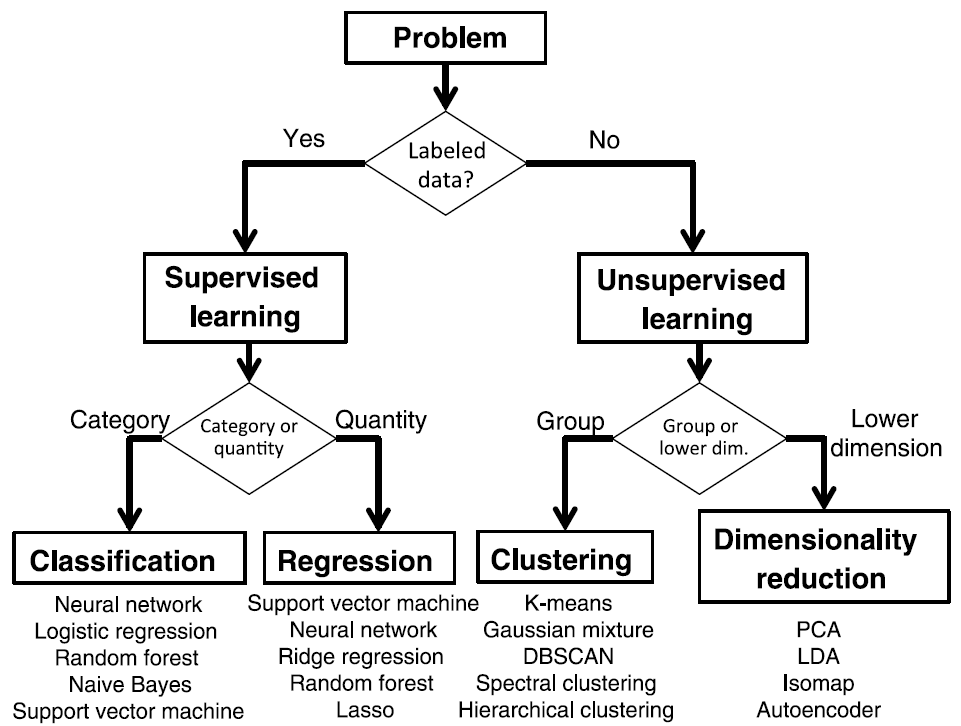
\includegraphics[width=0.6\textwidth]{MLtree.png}
\end{center}
\vspace{-0.3cm}

\subsection{The formalized set-up}
Imagine a data-set with samples and their label:
\begin{equation}
    \mathcal{D} = \Bigg\{ (\vec{x}_1,y_1), \dots, (\vec{x}_N,y_N) \Bigg\} \subseteq \mathcal{X}\times\mathcal{Y}
\end{equation}
where $\vec{x}_i$ is the $i$-th \textbf{feature vector} from space $\mathcal{X}$, and $y_i$ the corresponding \textbf{label} from space $\mathcal{Y}$. ($\mathcal{Y}$ could represent $k$ classes $\{0,1,\dots,k\}$ when we do a classification problem, or all real numbers $\mathbb{R}$ for a regression problem). We assume that the pairs are drawn i.i.d. from a distribution,
\begin{equation}
    (\vec{x}_i,y_i) \sim P,
\end{equation}
but this distribution is unknown to us!

Then we require a program (or `hypothesis'), referred to as $h(x)$ or $f(x)$ that maps $\vec{x}_i$ into $y_i$. We assume that the hypothesis $h$ is drawn from its own class $h\in\mathcal{C}$. Examples of the space $\mathcal{C}$ are decision trees, linear classifiers, artificial neural networks, support vector machines, \dots. The optimal algorithm is a problem-dependent feature. It often pays off to try a large number of methods (the `\textbf{No Free Lunch theorem}' states that there is no single optimal problem-independent algorithm).
\begin{spexample}[No Free Lunch theorem]
    The No Free Lunch (NFL) theorem states that there is no single algorithm that works optimally on \textit{all} problems. The contribution of NFL is that it tells us choosing an appropriate algorithm requires making assumptions about the kinds of target functions the algorithm is being used for. With no assumptions, no `meta-algorithm' performs better than random choice! In our case, it thus means that we should try a variety of models to see which model works optimally for our problem.
\end{spexample}

\subsection{Loss functions \& generalization}
To be able to distinguish between different hypotheses $h$, we require a scoring function that tells us `how well did my hypothesis perform for my data?'. This is provided by a \textbf{loss function} $L$, which tells us how \textit{badly} we predict a given set of samples.
\begin{spexample}[Loss-functions]
    \begin{enumerate}\itemsep0em
        \item \textbf{0-1 loss}. This loss function counts the number of wrong predictions:
        \begin{equation}
            L(h,\mathcal{D}) = \sum_{i=1}^N \mathbb{I}_{h(\vec{x}_i)\neq y_i}.
        \end{equation}
        \item \textbf{Squared loss}. For regression, it is more interesting to see how far off the true answer you are, which is typically measured with a squared loss function, weighing large errors extra:
        \begin{equation}
            L(h,\mathcal{D}) = \sum_{i=1}^N \lvert h(\vec{x}_i)-y_i \rvert^2.
        \end{equation}
        \item \textbf{Absolute loss}. Rather than the $L^2$-norm of the squared loss, we can consider an $L^1$-norm:
        \begin{equation}
            L(h,\mathcal{D}) = \sum_{i=1}^N \lvert h(\vec{x}_i)-y_i\rvert.
        \end{equation}
        In this setting, large errors will be less amplified -- you don't want the squared loss measure if large errors or statistical flukes are present in the training data (when big outliers are squared, they dominate the loss function's score fully, even if you do well on the rest!).
    \end{enumerate}
\end{spexample}
{\flushleft We} realize that loss-functions are \textbf{non-negative}, and the optimal solution lies at $L(h,\mathcal{D})=0$. However, note the following. If we train our data on a set of training data $\mathcal{Z}^\text{train}\subset\mathcal{D}$, and have the following simple hypothesis that just memorizes the input data:
\begin{equation}
    h^\bullet(\vec{x}) = \begin{cases} y_i & \text{if }\vec{x}=\vec{x}_i, \\ 0 & \text{otherwise}, \end{cases}
\end{equation}
it will have a loss-function $L(h^\bullet,\mathcal{Z}^\text{train})=0$, yet it will be terrible on any new inputs $\vec{x}$ not in the training data! Memorization would thus give a perfect loss function, but would not generalize at all! This is the problem that we must address: how do we design machine learning algorithms that generalize to \textit{all} samples drawn from $P$, not just the training samples!
\begin{testexample}[Generalization error for generals]
        \textsc{Kilian Weinberger} tells the humorous story of an image classifier that separated military from civilian vehicles, working really well on all collected data. But then it didn't work in practice at all! What happened was that all the military vehicles were photographed during the day, while the civilian vehicles were photographed much later in the day. Thus, the classifier simply learned that bright pictures were military vehicles, and the dark pictures were civilians! Clearly, the samples and reality were not drawn from a similar distribution $P$!
\end{testexample}

\subsection{Risk functions \& generalization}
So, we want to obtain a hypothesis $h$ that maps all relevant data inputs $\mathcal{X}$ to solutions $\mathcal{Y}$. However, $h$ can only trained on a subset $\mathcal{Z}^\text{train}\subset\mathcal{D}$, thus the difficulty lies in \textit{generalization}: how can we be sure that our hypothesis fits not only the training data but also new unseen data.
\begin{testexample}[Underfitting and overfitting]
    The goal in machine learning is to find a function that works well on \textit{all} relevant inputs, while only having a limited number of (noisy) training data available. Therefore, our optimal solution lies somewhere between an underfitting and overfitting solution:\\
    \begin{center}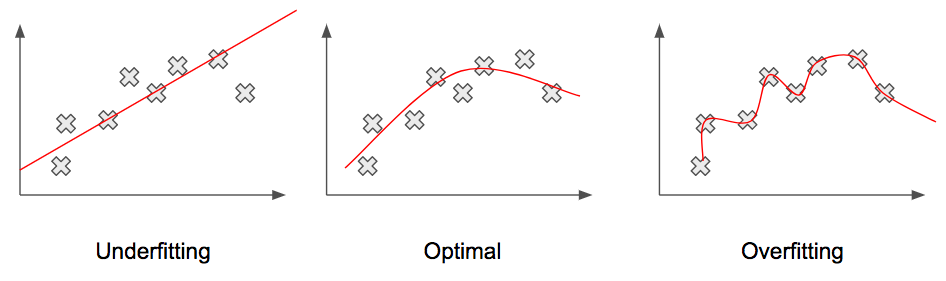
\includegraphics[width=0.7\textwidth]{Overfitting.png}\end{center}\vspace{-0.5cm}
\end{testexample}
{\flushleft Assume} that $\mathcal{Z}^\text{train}$ is drawn i.i.d. from the distribution $P$. Then choose a loss function $L(h,\mathcal{D}))$. We then define an \textbf{Expected risk function} that expresses the expected loss for \textit{all} data $\mathcal{D}$:
\begin{equation}
    R(h,\mathcal{D}) = \mathbb{E}[L(h,\mathcal{D})].\label{eq:exprisk}
\end{equation}
As an example, with the 0-1 loss-function we would obtain:
\begin{equation}
    R(h,\mathcal{D}) = \mathbb{E}[\mathbb{I}_{\hat{y}^\text{predicted}\neq y^\text{true}}].
\end{equation}
However, we can only compute the \textbf{Empirical risk function} (written with $R$-hat) based on the $N$ training data $\mathcal{Z}^\text{train}$, which simply equals the loss function equally weighted for all available data:
\begin{equation}
    \hat{R}(h,\mathcal{Z}^\text{train}) = \frac{1}{N} L(h,\mathcal{Z}^\text{train})\label{eq:emprisk}.
\end{equation}
As an example, with the 0-1 loss-function we would obtain:
\begin{equation}
    \hat{R}(h,\mathcal{Z}^\text{train}) =  \frac{1}{N}\sum_{i=1}^N \mathbb{I}_{h(x_i)\neq y_i}.
\end{equation}
If we just choose the function $h$ that minimizes the \textit{empirical risk function}, we're prone to obtain a hypothesis that is overfitting or just memorizes all the inputs. Often it holds that the optimal model $\hat{h}\in\argmin_h\hat{R}(h,\mathcal{Z}^\text{train})$ based on the training data overestimates the performance on all the data:
\begin{equation}
    \hat{R}(\hat{h},\mathcal{Z}^\text{train}) < R(\hat{h},\mathcal{D}).
\end{equation}
\begin{mymathbox}[ams align, title={Expected and Empirical Risk Functions}, colframe=blue!30!black, center title]
    R(h,\mathcal{D}) &= \mathbb{E}(L(h,\mathcal{D})),\\
    \hat{R}(h,\mathcal{Z}^\text{train}) &= \frac{1}{N}L(h,\mathcal{Z}^\text{train}).
\end{mymathbox}

\subsection{Generalization error \& holdout strategy}
Clearly, with only knowledge of the training data, it appears impossible to gain an understanding of the expected risk. However, an estimation of the risk can be made by splitting the available data in two. We keep a $N-M$ instances in the training data-set $\mathcal{Z}^\text{train}=(\mathcal{X}^\text{train}\times\mathcal{Y}^\text{train})$, and retain the remaining $M$ instances in a test data-set $\mathcal{Z}^\text{test}=(\mathcal{X}^\text{test}\times\mathcal{Y}^\text{test})$ which is held-out and only used to validate the results of the trained model, to compute the \textbf{test error}, for example with the 0-1 loss:
\begin{equation}
    \hat{R}(\hat{h},\mathcal{Z}^\text{test}) = \frac{1}{M}\sum_{m=1}^M \mathbb{I}_{\hat{h}(x_m)\neq y_m}.
\end{equation}
The test data-set should {\color{red}{\textbf{\textit{never}}}} be used within the training algorithm! The test error then gives an idea of the level of underfitting or overfitting, as it gives an estimate of the generalization error. Ideally, the model is tested only once on the test data -- for if one keeps tweaking the model to improve the score on the test data-set we are, in a complicated way, fitting our model to the test data-set as well! Therefore, it often also holds that the trained hypothesis $\hat{h}\in\arg\min \hat{R}(h,\mathcal{Z}^\text{train})$ still overestimates the expected risk, but is better already.
\begin{equation}
    \hat{R}(\hat{h},\mathcal{Z}^\text{test}) < R(\hat{h},\mathcal{D}).
\end{equation}

\begin{spexample}[Holdout strategy: Training, validation and test data]
    We established that if we choose the optimal hypothesis for our training data:
    \begin{equation}
        \hat{h} \in \argmin_{h}\hat{R}(h,\mathcal{Z}^\text{train}),
    \end{equation}
    we likely overfit and have a poor test-score, $\hat{R}(\hat{h},\mathcal{Z}^\text{test})$. Then how to fine-tune our model? Well -- we create \textit{another} split of the data: the \textbf{validation data}. This is equally held out during training like the test data, but is used to score various models immediately after the training; and the set of model `hyper-parameters' that optimize the \textbf{holdout score} become a good approximation of which model is most appropriate. Retraining on \textit{all} data with those optimal parameters then gives the final model, for which the test error may be computed.
    \begin{center}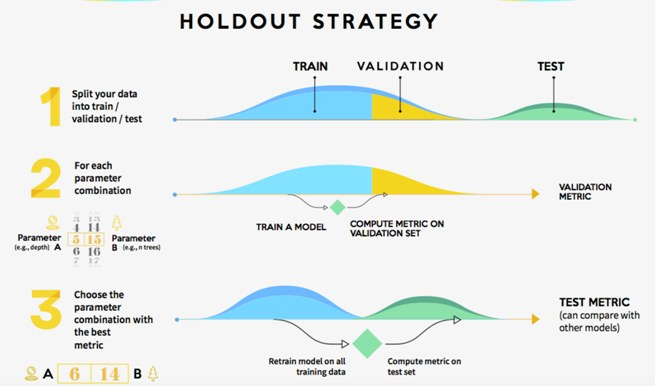
\includegraphics[width=0.8\textwidth]{holdout-strategy.jpg}\end{center}
\end{spexample}

\newpage
\section{Machine learning 102: Classification}
\subsection{Nearest neighbours}
\subsubsection{k-NN algorithm}
So, before going into the more statistical notions, a quick overview of the machine learning methods seems appropriate. The first method worth looking at is the ($k$-)nearest neighbour algorithm. The assumption is simple: similar inputs must have similar outputs. The the k-NN algorithm, for any test input $\vec{x}$, assigns it the most common label $y$ amongst its $k$ most similar training inputs. For example, in the below scenario we use $k=3$, yielding two blue points and one red point closest to the tested $\vec{x}$ (where we assign blue the $+1$ label and red the $-1$ label). This results in a majority predicting the label $+1$, which we may assign to $\vec{x}$ correspondingly:
\begin{center}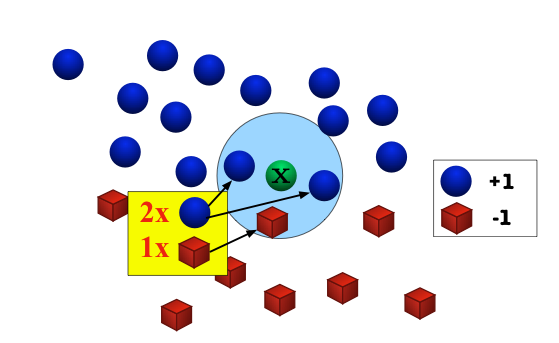
\includegraphics[width=0.4\textwidth]{knnfig.png}\end{center}

The positive aspect of the k-NN algorithm is simple and has a meaningful notion of (dis)similarity. The first downside of the method is that it is slow -- it needs to check the distance of one point against \textit{all} points in the training set! The second downside is that for a large-dimensional space (i.e., many features; a small 256$\times$256 black-and-white image has already 65\,536 individual pixel features!) the concept of closeness starts to break down. This is called the \textbf{curse of dimensionality}, and basically means that if you put 100 samples on a unit line $x\in[0,1]$, any random point will always lie close to another point, it is in other words `busy' on the line -- but in a $d$-dimensional space $\vec{x}\in[0,1]^d$ filled with 100 samples, most positions are \textit{not} taken and the data-space eventually consists almost entirely of points that are equally apart from each other! We require an exponential growth of training data to keep the feature-space filled with the same density, but that just slows down the algorithm even more...
\begin{center}
    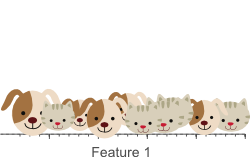
\includegraphics[width=0.3\textwidth]{1Dproblem.png}    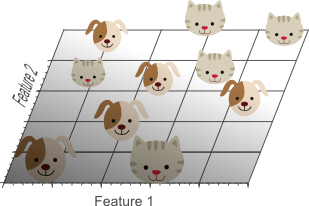
\includegraphics[width=0.3\textwidth]{2Dproblem.png}    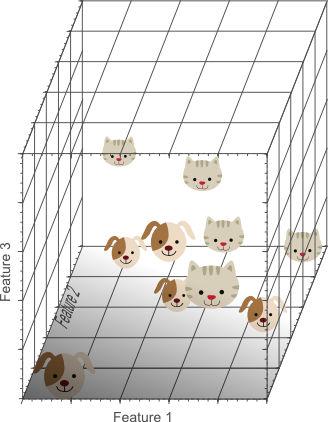
\includegraphics[width=0.3\textwidth]{3Dproblem.png}
\end{center}

\subsection{Separation by hyperplane}
We can also think of classification in the following way. Keeping things simple, we assume that there are two features and two states:
% \begin{figure}[H]
    % \centering
    \begin{center}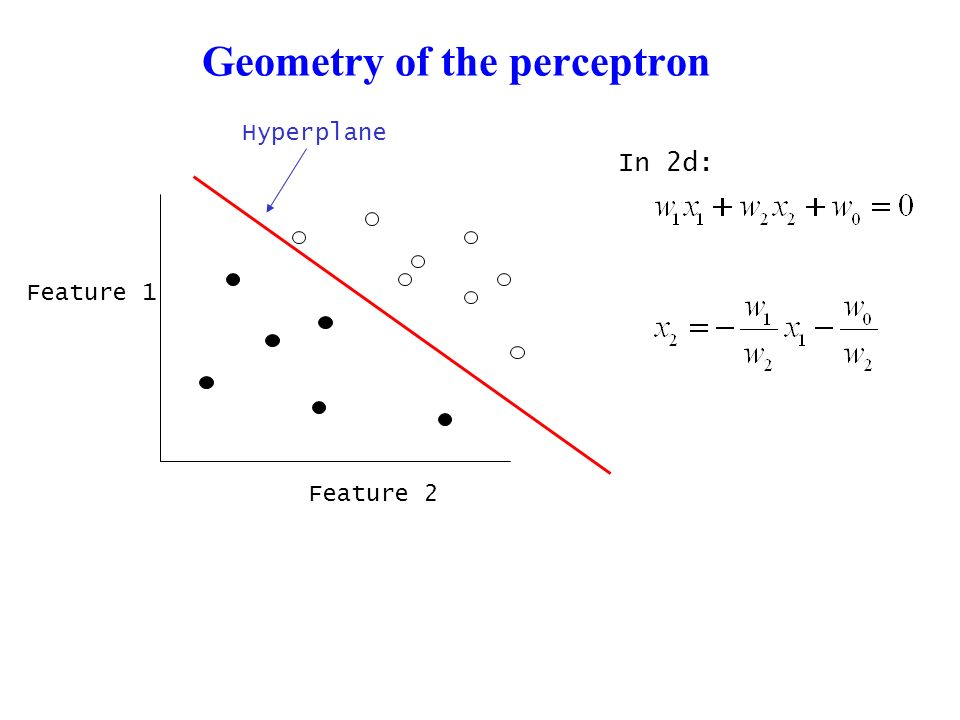
\includegraphics[width=0.5\textwidth,trim={0cm 6cm 10cm 3cm},clip]{perceptron_geometry.jpg}\end{center}
    % \caption{Caption}
    % \label{fig:my_label}
% \end{figure}
The classification problem is then really nothing more than \textit{finding the line that separates the two classes}! Because the data now lies on either side of the hyperplane, we can obtain this separator and then simply classify features based on their location in this feature space. We can take a more abstract notation, and choose to denote the feature vector $\vec{x}$ as:
\begin{equation}
    \vec{x} = \left[ \begin{array}{c} x_2 \\ x_2 \end{array}\right] = \left[ \begin{array}{c} \text{Feature 1} \\ \text{Feature 2} \end{array}\right]
\end{equation}
The red line that defines the hyperplane as we see it in the figure then looks something like:
\begin{equation}
    x_1 = \text{offset} - w_2x_2,
\end{equation}
where the `offset' defines how much $x_1$ we have when $x_2$ is zero, and $w_2$ defines the negative slope as we change $x_2$! Re-writing `offset' as $w_0$, we would obtain:
\begin{equation}
    x_1 = w_0 - w_2x_2,
\end{equation}
or more generally:
\begin{equation}
    w_0 + w_1x_1 + w_2x_2 = 0,
\end{equation}
which has the inner-product equation:
\begin{equation}
    \Big[\begin{array}{ccc} w_0 & w_1 & w_2 \end{array} \Big] \left[ \begin{array}{c} 1 \\ x_1 \\ x_2 \end{array} \right] = 0 \Longleftrightarrow \vec{w}^T\vec{x}^\bullet = 0
\end{equation}
Note that we augmented $\vec{x}$ to $\vec{x}^\bullet$ to absorb $w_0$! Note that the only variable here is $\vec{w}$, while $\vec{x}^\bullet$ is the same for any 2-D problem! The parameters of $\vec{w}$ thus define the entire classification problem. The classification, finally, is as simple as:
\begin{equation}
    h(\vec{x}_i^\bullet) = \begin{cases} \vec{w}^T\vec{x}_i^\bullet\geq 0 & \text{white class},\\ \vec{w}^T\vec{x}_i^\bullet<0 & \text{black class}.\end{cases}
\end{equation}

% \subsection{Classification algorithms}
\subsubsection{Perceptron}
The perceptron (\textsc{Rosenblatt}, 1957) is the first machine-learning algorithm that could learn to find a hyperplane based on the given data. We assume binary classes, positioned on the positive or negative side of the hyperplane:
\begin{equation}
    \mathcal{Y} = \{-1,+1\}.
\end{equation}
The perceptron then initializes with a random hyperplane parameterization $w^T$, takes a misclassified sample $(\vec{x}_i,y_i)$ (when $y_i\vec{w}^T\vec{x}_i\leq 0$) and adds it to the hyperplane with rule:
\begin{equation}
    w^T_\text{updated} = w^T + y_i \vec{x}_i^T
\end{equation}
Geometrically (the misclassified red box has $y=-1$, thus its location is subtracted from $w^T$):
\begin{center}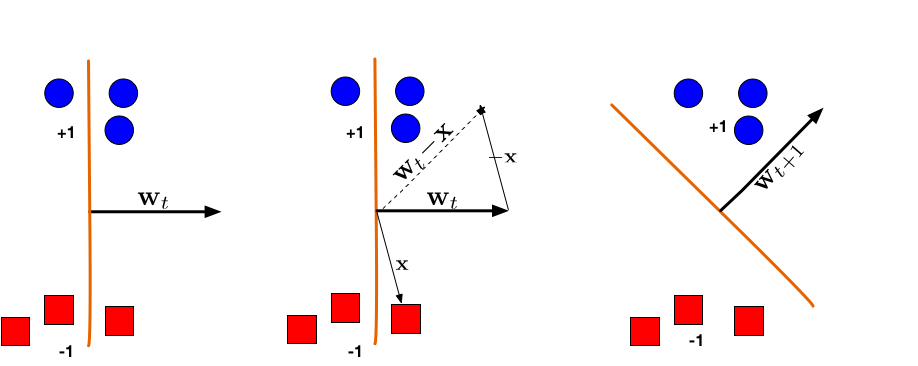
\includegraphics[width=0.9\textwidth,trim={0cm 0cm 3.2cm 2cm},clip]{PerceptronUpdate.png}\end{center}
The resulting hyperplane is often illustrated with a graph, which realizes a single \textit{output} of the algorithm:
\begin{center}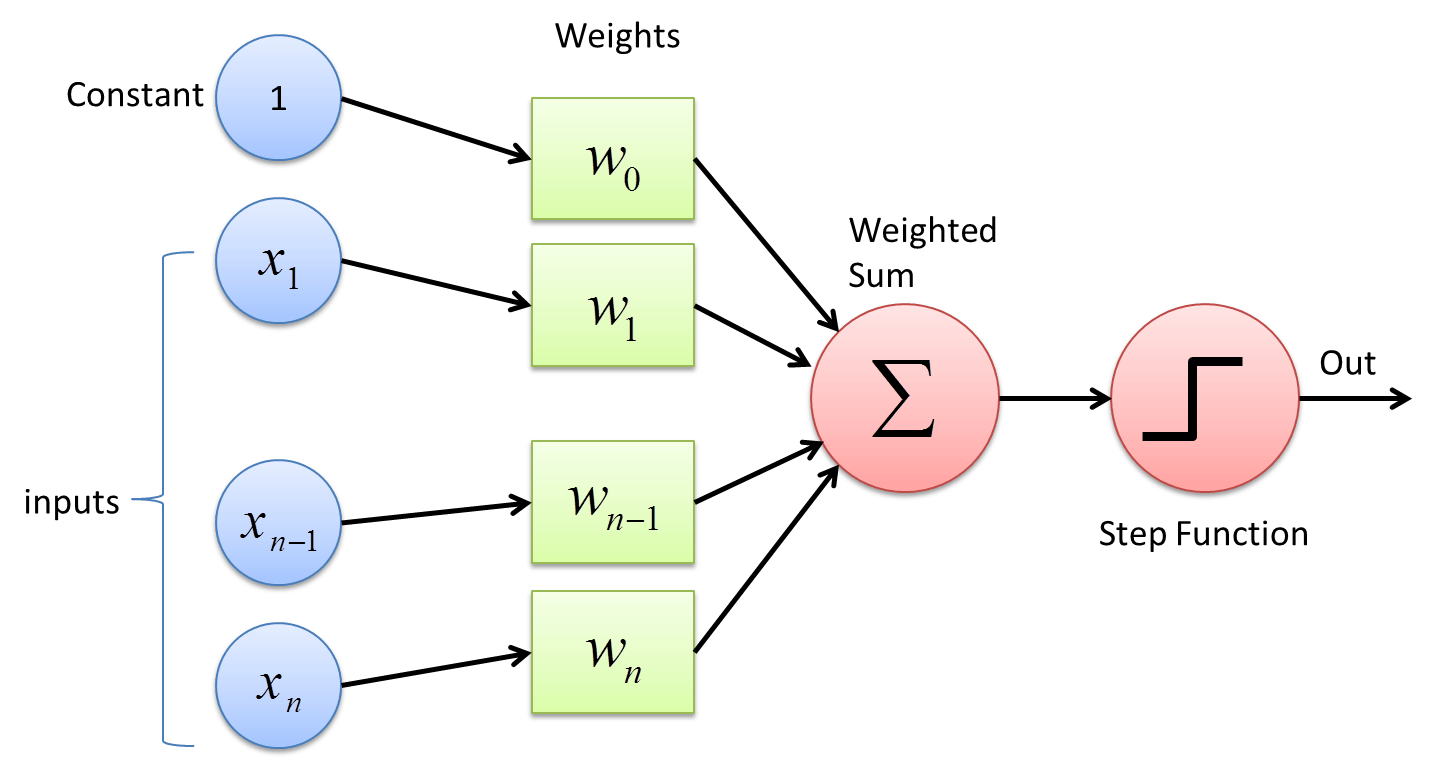
\includegraphics[width=0.8\textwidth]{perceptrongraph.png}\end{center}
Note that the figure really just expresses this mathematical operation: $\sign(\vec{w}^T\vec{x}^\bullet_i)$. For a given input $\vec{x}$ and a constant we obtain $\vec{x}^\bullet_i$, and weights $\vec{w}$ are established, we compute the `weighted sum' (the scalar product $\vec{w}^T\vec{x}^\bullet_i$), and a step function is used to see whether the outcome is positive or negative ($\sign(\vec{w}^T\vec{x}^\bullet_i)$).

\begin{testexample}[Handwritten number recognition]
    The method appeared to work rather well for recognition of handwriting also, considering every pixel as an entry of the vector $\vec{x}$, which multiplied with the weights $\vec{w}$ separate a 0 from a 7:
    \begin{center}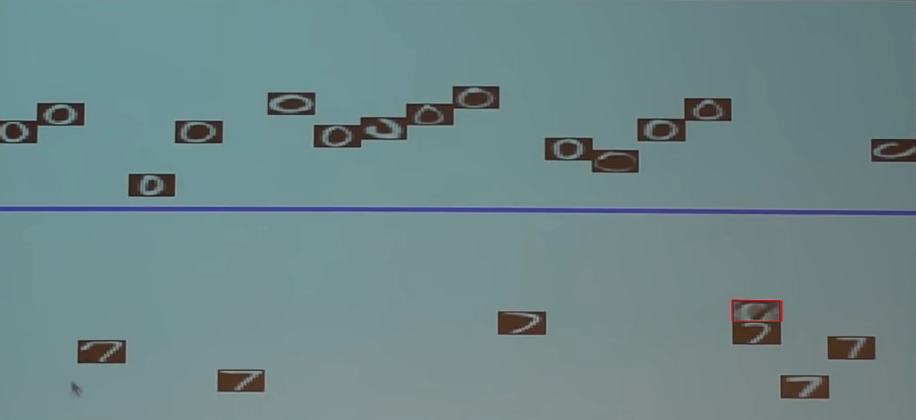
\includegraphics[width=1\textwidth]{numberrecog.png}\end{center}
    The weights are illustrated in red outline, on top of the `7' fourth of the right. You see that you can discern a white 0 and a black 7 in the weight. Thus multiplying a white zero image with the white `0' weight, and summing over the result, gives a positive sum; while multiplying a white 7 with the black `7' weight sums to a negative result. Thus: the two data are separated by their score after summation between image and weight!
\end{testexample}



\subsubsection{Support vector machines}
The perceptron doesn't guarantee that it finds a \textit{good} separating hyperplane; in fact there is an infinite number of hyperplane variations that all work. The support vector machine (\textsc{Vapnik \& Chervonenkis}, 1963) tries to obtain the separating hyperplane that \textit{maximizes} the distance (`margin') between the two clusters. In practice, that means that we can draw two parallel lines (one running through two points of a class, and another one through a single point from the other class, called the `support vectors'). The line exactly in-between the parallel vectors gives the separator with the largest possible margin:
\begin{center}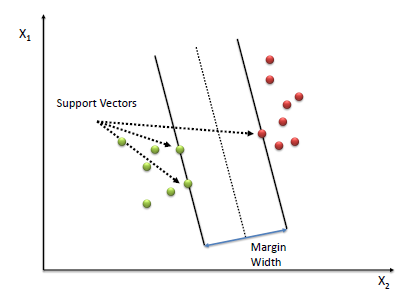
\includegraphics[width=0.47\textwidth]{SVM.png}\end{center}

\subsubsection{The kernel trick}
The ability to make linear separation boundaries only is rather limiting. But extending the previous methods to other separation boundaries is difficult -- they are so inherently based on ideas of linearity. The trick that came about is the `Kernel method', by which the data is transformed into another space, after which the data becomes linearly separable. One example keeps the features in the same dimensions:
\begin{center}
    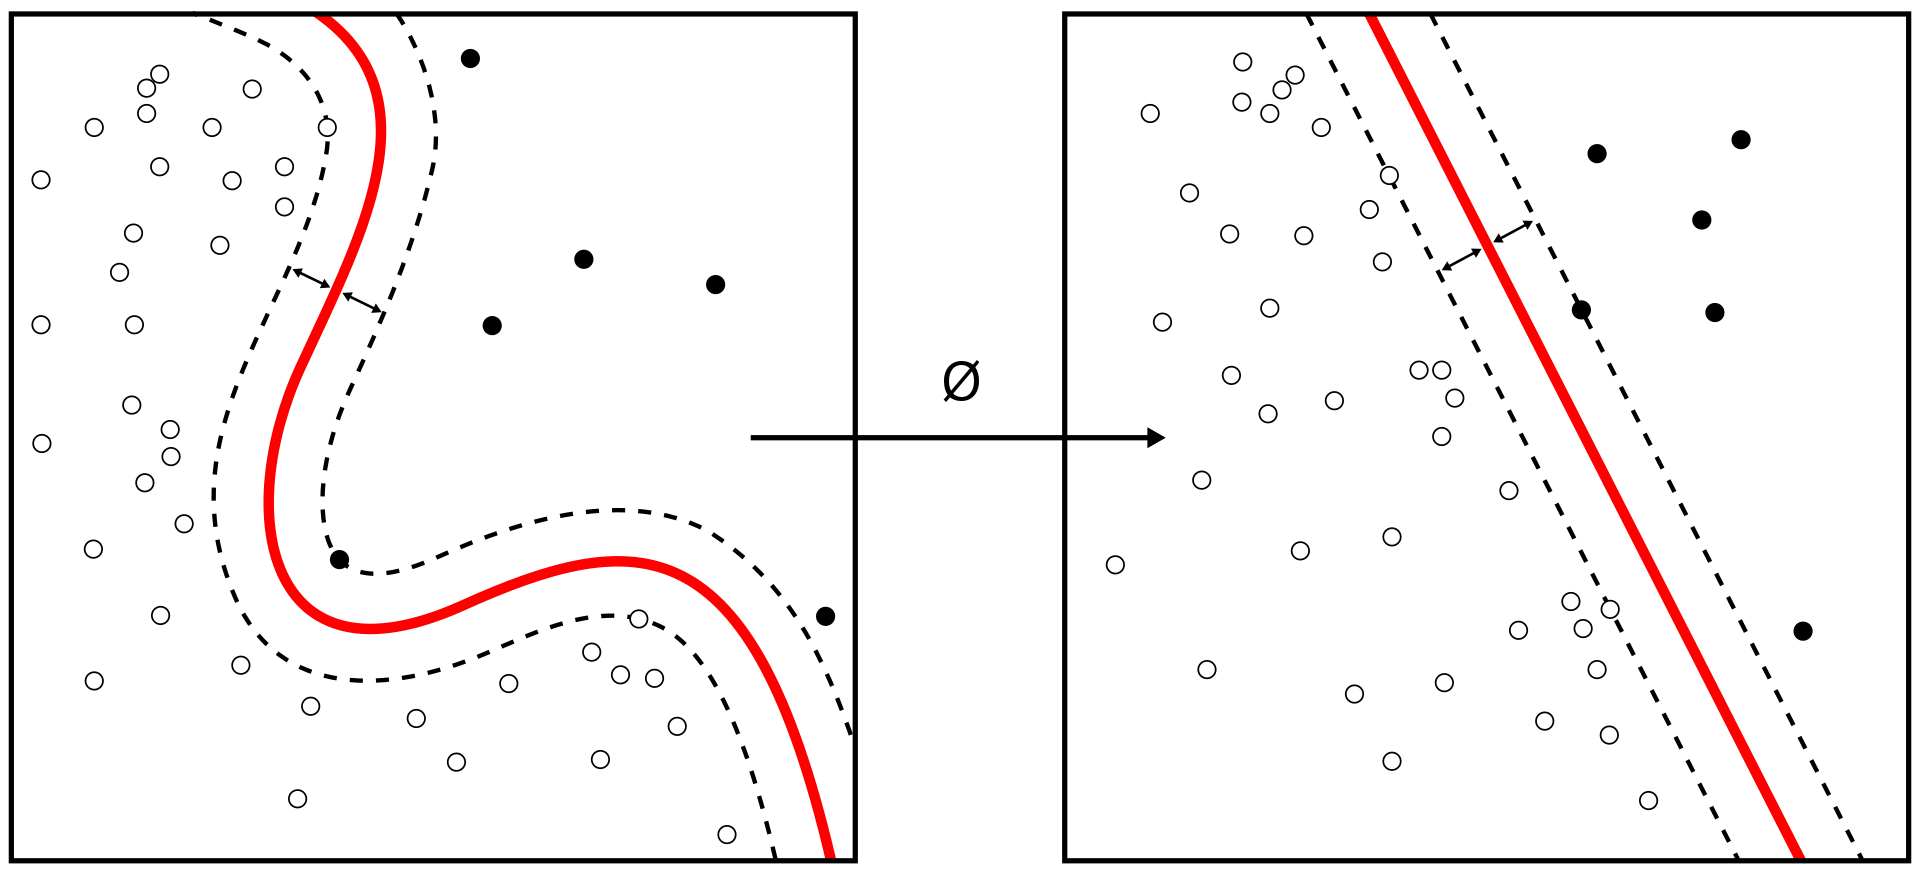
\includegraphics[width=0.6\textwidth]{kernel.png}
\end{center}
but a more common example is to add an additional dimension to the feature space, allowing strongly non-linear feature maps:
\begin{center}
    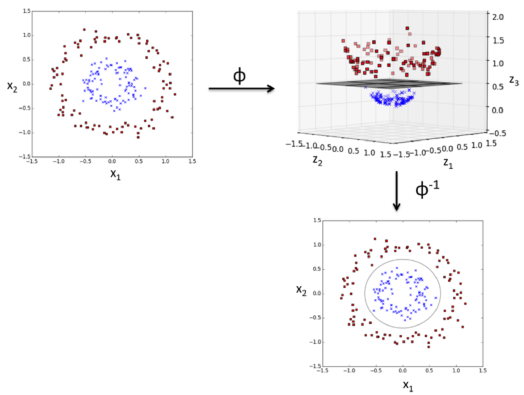
\includegraphics[width=0.6\textwidth]{kernel-method-nonlinear-svm.png}
\end{center}
The crucial portion is that the SVM optimization minimizes a quadratic term that involves the scalar product of the data $\vec{x}^T\vec{x}$, and its coordinate transformed version is $\phi(\vec{x})^T\phi(\vec{x})$. To compute the latter term requires expanding the vector into a usually higher-dimensional space $\phi(\vec{x})$, and then the scalar product collapses this back to a scalar again. The `kernel method', on the other hand, never leaves the original feature space explicitly, by computing the scalar product of the transformations beforehand, $K=\phi(\cdot)^T\phi(\cdot)$. This allows us to obtain the scalar-product immediately through $K(\vec{x})$! Effectively, as long as you choose an appropriate kernel (Gaussian radial basis functions are the most popular one, which transform into an \textit{infinite}-dimensional space!) you can now also fit non-linear clusters extremely rapidly with your linear algorithm.

\newpage
\subsection{Probabilistic models}
We can take yet another look at the problem, from probabilistic perspective. Assume that the data $\mathcal{Z}^\text{train}=(\mathcal{X}^\text{train}\times\mathcal{Y}^\text{train})$ can be explained by a certain distribution, parameterized with $\theta$. We can then fit the distribution to our data, and then predict any point by evaluating the simple rules of probability. Compared to the previous two methods (nearest neighbour and separating hyperplane), we now actually obtain the computed \textit{probability} that any point belongs to either of the clusters!

\subsubsection{Maximum Likelihood Estimation (MLE)}
The rule is simple. For training, we try to find the best parameter that explains the data. So for the parameter $\theta$, we express the likelihood of finding any combination (i.e., joint probability distribution) of data $\mathcal{Z}^\text{train}$ and parameter $\theta_j$ (one parameter for each class $j$), and we want to find the $\theta_j$ that maximizes this probability:
\begin{equation}
    \hat{\theta}_j\in\argmax_\theta \mathbb{P}(\mathcal{Z}^\text{train}|\theta_j) = \argmax_\theta \log\left( \mathbb{P}(\mathcal{Z}^\text{train}|\theta_j) \right).
\end{equation}
Once we have found the $\theta$ that optimally fits the distributions in the data, we can create plots like below which consists of multivariate Gaussians:
\begin{center}
    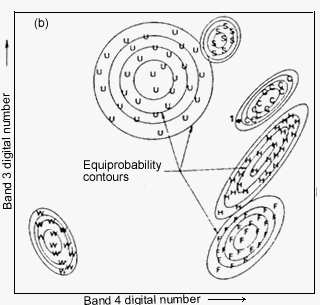
\includegraphics[width=0.6\textwidth,trim={0.5cm 0.35cm 0 0},clip]{MLE_class.jpg}
\end{center}
Because we now know the underlying distributions, we can simply find the probability of any new data point, and for example assign the new point to the most probable class $j$:
\begin{equation}
    \argmax_j \mathbb{P}(\vec{x}|\hat{\theta}_j).
\end{equation}
Finding the optimal $\hat{\theta}$ is actually a fairly hard problem to solve directly, but iterative methods like the `Expectation and Maximization' (EM) algorithm exist to obtain these methods instead. This method  When using strictly Normal distributions, the obtained model is called a `Gaussian Mixture Model' (GMM).

\subsubsection{Naive Bayesian}
The Naive Bayesian classifier assumes that there is no covariance between the features. This simplifies the method and is furthermore rather robust in practice! You can see it in this plot because the Gaussians are aligned with the grid, not allowed to rotate as we saw on the previous page.
\begin{center}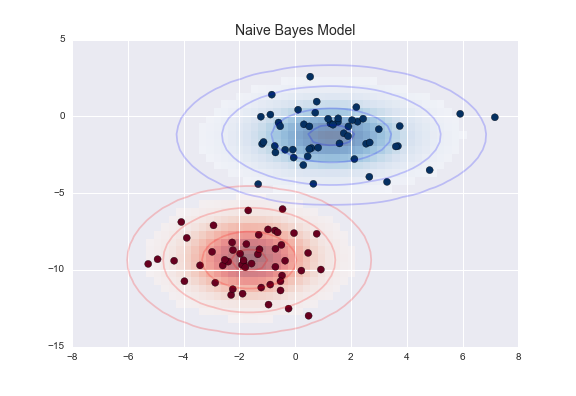
\includegraphics[width=0.8\textwidth]{naivegaussian.png}
\end{center}



\subsubsection{Maximum a posteriori (MAP)}
Rather than optimizing for the likelihood only, we can find the a posteriori solution instead, which happens to give us a way to weigh specific distributions favourably or not:
\begin{equation}
    \hat{\theta}_j\in\argmax_{\theta_j} \mathbb{P}(\theta_j|\mathcal{Z}^\text{train}) = \argmax_{\theta_j} \frac{\mathbb{P}(\mathcal{Z}^\text{train}|\theta_j)\mathbb{P}(\theta_j)}{\mathbb{P}(\mathcal{Z}^\text{train})} = \argmax_{\theta_j} \mathbb{P}(\mathcal{Z}^\text{train}|\theta_j)\mathbb{P}(\theta_j),
\end{equation}
the latter form follows because there is no dependency on $\theta$ in the evidence, i.e., it plays no role in the optimization. The resulting form thus weighs the probability we saw earlier in the MLE method, by the probability of observing $\theta_j$ at all! This prior $\mathbb{P}(\theta_j)$ is independent of the data and we can consider it to be a form of \textbf{regularization}: when the parameter $\theta_j$ deviates much from what we believe is reasonable, we need a lot of evidence to convince us it's right.

The MAP thus reduces the MLE if we assume a uniform prior for the parameters $\theta_j$!

\begin{mymathbox}[ams align, title={MLE \& MAP}, colframe=blue!30!black, center title]
    \text{MLE:}\quad & \argmax_{\vec{w}} \mathbb{P}(\mathcal{Z}^\text{train}|\vec{w})=\argmax_{\vec{w}} \prod_{n=1}^N \mathbb{P}(y_i|x_i,\vec{w})= \argmax_{\vec{w}}\prod_{n=1}^N \mathcal{N}(\vec{w}^T\vec{x},\sigma^2), \\
    \text{MAP:}\quad & \argmax_{\vec{w}}\mathbb{P}(\vec{w}|\mathcal{Z}^\text{train})\propto \mathbb{P}(\mathcal{Z}^\text{train}|\vec{w}))\mathbb{P}(\vec{w}).
\end{mymathbox}

% \begin{spexample}[MLE coin throws]
%     Assume we flip the same coin repeatedly, we have a constant $\mathcal{X}^\text{train}$ but a binary outcome $\mathcal{Y}^\text{train}$. For example, $\mathcal{Y}^\text{train}=\{H,T,T,H,H,H,T,T,T,T\}$. We thus know a binomial distribution applies:
%     \begin{align}
%         \hat{\theta} = \argmax_\theta \log\left[ \mathbb{P}(\mathcal{Y}^\text{train},\theta)\right]&= \argmax_\theta \log\left[ \binom{\#H+\#T}{\#H}+\theta^{\#H}(1-\theta)^{\#T} \right],\\
%         &=\argmax_\theta \#H\log[\theta]+\#T\log[1-\theta]
%     \end{align}
% \end{spexample}

\newpage
\section{Machine learning 103: Regression}
\subsection{Least-squares}
If we assume that a linear regression relation exists (knowing that with the kernel trick from above, we can make things work for non-linear models also), we assume that input feature $\vec{x}$ has $d$ dimensions:
\begin{equation}
    y = w_0 + \sum_{j=1}^d x_j w_j,
\end{equation}
or using homogeneous coordinates again ($x^\bullet=[1\ x]^T$), the linear function has a familiar form:
\begin{equation}
    y = \vec{w}^T\vec{x}^\bullet = \vec{x}^{\bullet T}\vec{w}.\label{eq:standardlinearform}
\end{equation}
We now again have various choices of methods that can give us the optimal weights $w$. For example, the \textbf{least-squares method} (or `residual sum of squares') tries to obtain, based on all $N$ pairs of $(x_i,y_i)$, the optimal weights:
\begin{equation}
    \widehat{w} = \argmin_{\vec{w}} \sum_{i=1}^N (y_i - \vec{w}^T\vec{x}^\bullet_i)^2 = \argmin_{\vec{w}} (\mathbf{y}-\mathbf{\vec{x}}\vec{w})^2 = \argmin_{\vec{w}} \norm*{\mathbf{y}-\mathbf{\vec{x}}\vec{w}}_2^2,
\end{equation}
with vector $\mathbf{y}=[y_1\ y_2\ \dots\ y_N]^T$ and matrix $\mathbf{\vec{x}}=[\vec{x}_1^{\bullet}\ \vec{x}^{\bullet}_2\ \dots\ \vec{x}^{\bullet}_N]^T$ this has the optimal solution:
\begin{equation}
    \widehat{w} = (\mathbf{\vec{x}}^{T}\mathbf{\vec{x}})^{-1} \mathbf{\vec{x}}^{T}\mathbf{y}.
\end{equation}
There is much more to say about these solutions, but I'll leave that for later.

\begin{spexample}[Regularization models]
    If we think we know more about $\widehat{w}$, i.e., we have a prior, we can regularize the inversion. For example, with \textbf{Ridge Regression} we simultaneously triy to minimize the `energy' in the misfit, as well as in the weights vector itself:
    \begin{equation}
        \widehat{w} = \argmin_{\vec{w}} \norm*{\mathbf{y}-\mathbf{\vec{x}}\vec{w}}_2^2 + \lambda\vec{w}^T\vec{w} = \argmin_{\vec{w}} \norm*{\mathbf{y}-\mathbf{\vec{x}}\vec{w}}_2^2 + \lambda\norm*{\vec{w}}_2^2,
    \end{equation}
    which has the explicit solution:
    \begin{equation}
        \widehat{w} = (\mathbf{\vec{x}}^T\mathbf{\vec{x}}+\lambda\mathbf{I})^{-1}\mathbf{\vec{x}}^T\mathbf{y}.
    \end{equation}
    
    Conversely, in \textbf{LASSO} (Least Absolute Shrinkage and Selection Operator) regression, we simultaneously try to minimize the `energy' in the misfit and furthermore try to achieve a sparse weights vector:
    \begin{equation}
        \widehat{w} = \argmin_{\vec{w}} \norm*{\mathbf{y}-\mathbf{\vec{x}}\vec{w}}_2^2 + s\norm*{\vec{w}}_1^2.
    \end{equation}
    There is no explicit solution for this (often encountered in engineering problems) model, but efficient optimization techniques exist to solve this problem. The weights from the LASSO optimization usually result in only a few non-zero coefficients.
\end{spexample}
We can now write down the linear, least-squares regression model by inserting the optimal solution in eq. \eqref{eq:standardlinearform} to predict any new solution:
\begin{equation}
    \underbrace{y}_\text{new prediction} = \underbrace{\left((\mathbf{\vec{x}}^{T}\mathbf{\vec{x}})^{-1} \mathbf{\vec{x}}^{T}\mathbf{y}\right)^T}_\text{training data}\underbrace{\vec{x}^\bullet}_\text{new data}.
\end{equation}

\subsection{Bayesian regression}
We make a slightly altered assumption by explicitly incorporating  a noise coefficient $\epsilon$ from a parameterized distribution into our regression model, for example following a normal distribution:
\begin{equation}
    y = \vec{x}^{\bullet T}\vec{w} + \epsilon\quad\quad\text{with }\epsilon \sim \mathcal{N}(\epsilon|0,\sigma).
\end{equation}
This can also be written as a probability function:
\begin{equation}
    \mathbb{P}(y|\vec{x},\vec{w},\sigma) = \mathcal{N}(y|\vec{x}^{\bullet T}\vec{w},\sigma), \Longleftrightarrow y \sim \mathcal{N}(\vec{x}^{\bullet T}\vec{w},\sigma),\label{eq:drawingy}
\end{equation}
that is, the `mean' of every $y$ is given by the linear relation we saw in eq. \eqref{eq:standardlinearform}, but it is polluted with a normally distributed variance term $\sigma^2$. For $\sigma\to 0$ this is thus a straight line, but for larger $\sigma$, we obtain a whole range of possible realizations $y$, depending on the exact $y$ drawn from this normal distribution! We thus also obtain a \textit{range} of possible linear fits based on the data -- not necessarily the same as the ordinary least-squares (OLS) solution!
\begin{center}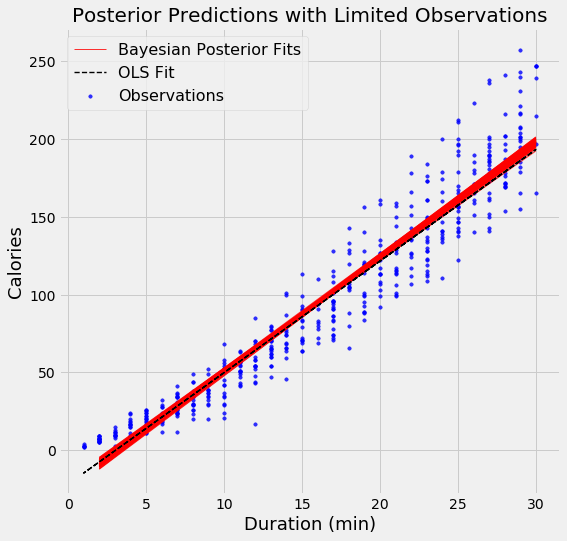
\includegraphics[width=0.5\textwidth]{bayeslinearregression.png}\end{center}


However -- we don't know the weights $\vec{w}$ yet. But we can find these as a data-conditional probability. For example, assuming the ridge-regression prior on $\vec{w}$ given in the previous section, we assume a multivariate distribution (dimension $d$, the size of the weights vector):
\begin{equation}
    \mathbb{P}(\vec{w}|\lambda\mathbf{I}) = \mathcal{N}(\vec{w}|0,(\lambda\mathbf{I})^{-1}) = \frac{\sqrt{\lambda^d}}{\sqrt{(2\pi)^d}}e^{-\frac{\lambda \vec{w}^t\vec{w}}{2}}.
\end{equation}
Then we can use Bayes' theorem to obtain the posterior, given the data:
\begin{equation}
    \mathbb{P}(\vec{w}|\mathbf{\vec{x}},\mathbf{y},\lambda\mathbf{I}) = \frac{\mathbb{P}(\mathbf{\vec{x}},\mathbf{y}|\vec{w},\lambda\mathbf{I})\mathbb{P}(\vec{w}|\lambda\mathbf{I})}{\mathbb{P}(\mathbf{\vec{x}},\mathbf{y}|\lambda\mathbf{I})} = \mathcal{N}(\vec{w}|\underbrace{(\mathbf{\vec{x}}^T\mathbf{\vec{x}}+\lambda\mathbf{I})^{-1}\mathbf{\vec{x}}^T\mathbf{y}}_{\mu_w},\underbrace{(\mathbf{\vec{x}}^T\mathbf{\vec{x}}+\lambda\mathbf{I})^{-1}}_{\Sigma_w}),
\end{equation}
that is, we compute how likely it is to arrive at model $\vec{w}$ given the data and an estimate of the form of $\vec{w}$. The solution we find is that there is an average $\vec{w}$ given by $\mu$ which equals the Ridge Regression solution, but additionally there is a variance of additional possible $\vec{w}$ values with the given variance $\Sigma$. That is, we can draw realizations of $\widehat{w}$ from the found probability distribution:
\begin{equation}
    \widehat{w} \sim \mathcal{N}(\vec{w}|\mu_w,\Sigma_w).
\end{equation}

Using the Kernel trick we can, furthermore, stray away from strictly linear regression, assuming the data is transformed:
\begin{equation}
    y = \vec{w}^T\phi(x)+\epsilon.
\end{equation}
\begin{center}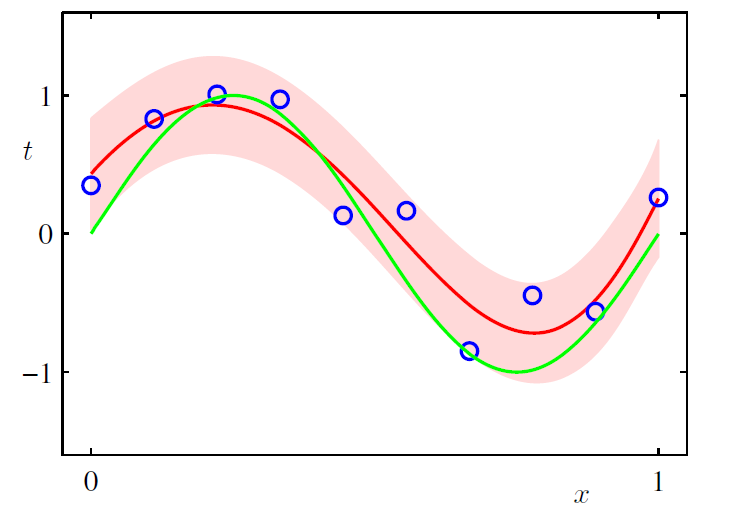
\includegraphics[width=0.5\textwidth]{bishop.png}\end{center}

\begin{mymathbox}[ams align, title={Regression models (so far)}, colframe=blue!30!black, center title]
    y & = \vec{w}^T\vec{x}+\epsilon,&&\text{Least-squares, ridge regression, linear Bayes regression},\\
    y & = \vec{w}^T\phi(\vec{x})+\epsilon&&\text{Kernelized regression}
\end{mymathbox}


\subsection{Gaussian process}
In the previous section, eq. \eqref{eq:drawingy}, we assumed that each $y$ was drawn from a linear line with some variability in exact $y$ value. In the Gaussian process, we assume that each output $y_i$ is potentially correlated with each other output $y_j$. Furthermore, we allow the regression model to be absolutely \textit{anything}:
\begin{equation}
    y = f(\vec{x})+\epsilon.
\end{equation}
Basically, the idea is that we are almost \textbf{model-independent}, make no choice for the data at all ($\vec{w}$ and $\phi$), and want to make predictions based on the actual training data itself. Remembering the MLE and MAP solutions from classification before, we now have a look with a Bayesian hat:
\begin{mymathbox}[ams align, title={MLE \& MAP}, colframe=blue!30!black, center title]
    \text{MLE:}\quad & \argmax_{\vec{w}} \mathbb{P}(\mathcal{Z}^\text{train}|\vec{w})=\argmax_{\vec{w}} \prod_{n=1}^N \mathbb{P}(y_i|x_i,\vec{w})= \argmax_{\vec{w}}\prod_{n=1}^N \mathcal{N}(\vec{w}^T\vec{x},\sigma^2), \\
    \text{MAP:}\quad & \argmax_{\vec{w}}\mathbb{P}(\vec{w}|\mathcal{Z}^\text{train})\propto \mathbb{P}(\mathcal{Z}^\text{train}|\vec{w}))\mathbb{P}(\vec{w}),\\
    \text{GP:}\quad& \mathbb{P}(y_\text{prediction}|x_\text{new},\mathbb{Z}^\text{train})=\int_{\vec{w}} \mathbb{P}(y|x,\vec{w})\mathbb{P}(\vec{w}|\mathcal{Z}^\text{train})\di\vec{w}. 
\end{mymathbox}
Hence, we marginalize out the model completely, with the last term equaling the one we saw in MAP. You never have to find a single set of parameters that represent the model for you, because you marginalize over all possible models in the universe! We don't commit to a single model, we simply assume \text{all} possible lines that we can draw are possible models, and we let the data constrain the type of models that actually work for our data! In the figure below, we thus have some \textit{priors} (all possible models in the universe, only assuming some smoothness between data points), then some draws from the \textit{posterior} (all possible models in the universe from the prior that cross through the known data at $x=\{2,4,6,7,9\}$), which we can also graph in the way that is done in the right-most picture that shows the standard-deviation of those models:
\begin{center}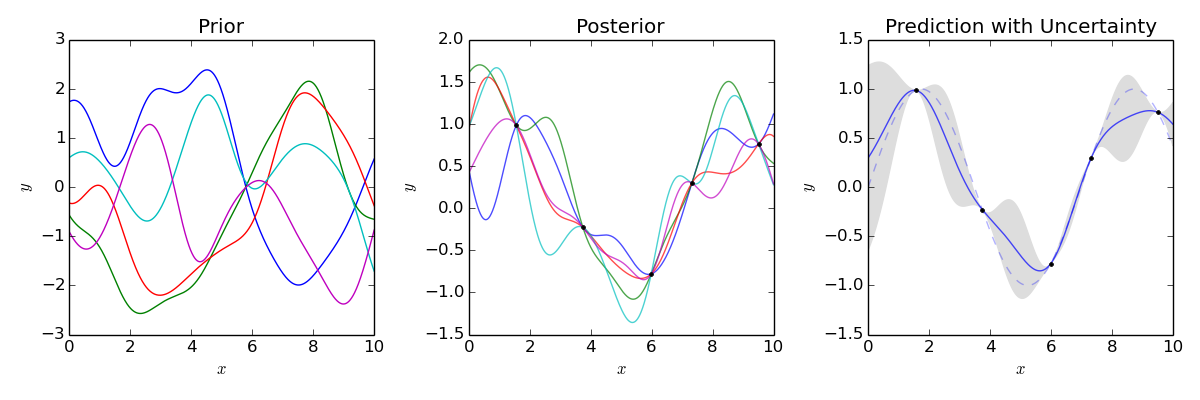
\includegraphics[width=0.8\textwidth]{Gaussian_Process_Regression.png}\end{center}
The only required input is thus the \textit{covariance} or \textit{Kernel} function that expresses the smoothness of the prior models -- i.e., how smooth or spiky are the lines that we consider in our prior. Check out the demos: \url{https://youtu.be/R-NUdqxKjos?t=2829} and  \url{https://youtu.be/BzHJ57QCdVo?t=945}.

The great thing is that the entire formulation of the Gaussian Process (GP) in the box above is just integrating over multiplications of Gaussians, so we know that the solution is also a Gaussian itself. Therefore, any point in the solution space is simply the result of a (multivariate) Gaussian fitting procedure, where we assume that for any known data-point, it tells us something about the values corresponding to data close by. Hence, in the figure you see that close to any data-point, the fit is extremely good, but gets more uncertain further away. 

In other words, we assume that our `known' values $\mathcal{Y}^\text{train}$, as well as our latest new value $y_N$ are drawn from a multivariate Gaussian distribution:
\begin{equation}
    \left[ \begin{array}{c} \mathcal{Y}_1 \\ \mathcal{Y}_2 \\ \vdots \\ y_N \end{array} \right] \sim \mathcal{N}\left( \mathbf{y} \Bigg| \mathbf{0}, \left[ \begin{array}{cccc} k_{1,1}+\sigma^2 & k_{1,2} & \dots & k_{1,N} \\ k_{2,1} & k_{2,2}+\sigma^2 & \dots & k_{2,N} \\ \vdots & \vdots & \ddots & \vdots \\ k_{N,1} & k_{N,2} & \dots & k_{N,N}+\sigma^2 \end{array} \right] \right)\label{eq:gppdistribution}
\end{equation}
Where $k_{i,j}$ represents the kernel that represents something like the covariance between points $x_i,x_j$. For the \textbf{diagonal terms}: If $k_{i,i}+\sigma^2=0$, every draw from the distribution in eq. \eqref{eq:gppdistribution} returns exactly the previously sampled points of $\mathcal{Y}^\text{train}$! Allowing $k_{i,i}+\sigma^2>0$, there is allowed to be some error even in drawing realizations from the posterior. For the \textbf{off-diagonal terms}: If $k_{i,j}$ is large, the values $\mathcal{Y}_i$ and $\mathcal{Y}_j$ will be similar, because they are correlated with each other.

Your choice of $k$ is where the assumption comes in (the No Free Lunch Theorem!), and where you have to make a choice. A typical kernel is the `Gaussian' kernel:
\begin{equation}
    k_{i,j} = e^{-\frac{-|x_i-x_j|^2}{\sigma_f}},
\end{equation}
where $\sigma_f$ is a chosen hyperparameter.


It is interesting to think of the various options as taking two steps in the least-squares and Bayesian regression learning (learning the model, then making new predictions, i.e., induction and then deduction); while the Gaussian Process goes straight from the known data to the new predictions (i.e., transduction).
\begin{center}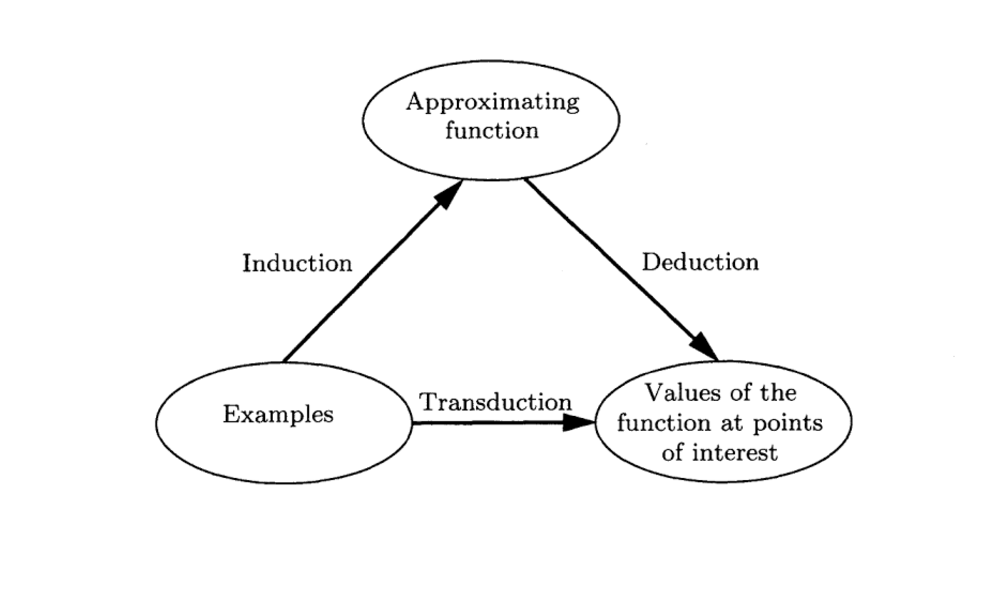
\includegraphics[width=0.8\textwidth]{indetransudction.png}\end{center}

% \newpage

\section{Machine Learning 104: Density Estimation}
I'll keep this short because there is not much to say. But if the data is unstructured, i.e., there are no available $y$ outcomes and we merely wonder about \textit{where} clusters are or \textit{how many} clusters there are, there are various methods we can try. Principally, we discussed \textbf{four} methods. The \textbf{expectation-maximization (EM) method} which clusters data into a given number of clusters; and the \textbf{Latent Dirichlet Allocation (LDA)} which clusters data into a non-prior given number of clusters, i.e., it is a fully data-driven process. The \textbf{Generative Adversarial Network (GAN)} learns how to cluster the data in an unspecified number of clusters; and plays a game against itself with two neural networks -- one creates samples from, approximately, the same distribution as the input data, and the other neural network must distinguish real data from made-up data; a \textit{generator} and a \textit{discriminator}. The \textbf{Autoencoder} learns to decode the original structure into a lower-dimensional form and reconstruct it back from there using two mirrored neural networks. The latter option is not dissimilar from \textbf{PCA}, in the sense that it finds a lower-dimensional structure in higher-dimensional data.


\newpage

\section{Machine learning 201: Quantifying Accuracy}
\subsection{Bias-variance trade-off of expected risk}
The \textbf{bian-variance trade-off} is a defining insight that separates the people just playing around with algorithms from the data-scientists. We simply decompose the \textbf{test-error} into a squared bias term, a squared error term and a squared deviation (thus, variance) term. We assume a training data-set of $N$ entries as drawn from:
\begin{equation}
    \mathcal{Z}^\text{train}\sim \mathbb{P}(X,Y)^N,
\end{equation}
as well as a new test-point $\{x,y\}$ drawn from the same distribution:
\begin{equation}
    \{x,y\}\sim \mathbb{P}(X,Y).
\end{equation}
It is important to realize that $\mathcal{Z}^\text{train}$ and $\{x,y\}$ are \textit{independent random variables} drawn from the distribution $\mathbb{P}(X,Y)$.

Furthermore, we understand that (the training data and new test-point being random variables), we can have do expectations over them that give averages, denoted with a bar. We require $\overline{y}$ and $\overline{h}_\mathcal{Z}$ for our purpose. We can find the average outcome, given $x$, i.e. a relationship $y(x)$:
\begin{equation}
    \overline{y}(x) = \mathbb{E}_{y|x}[Y].\quad\text{\textbf{Expected label}}.
\end{equation}
Furthermore, assume we have some algorithm that produces classifiers based on input data $\mathcal{Z}$:
\begin{equation}
    \overline{h}(x) = \mathbb{E}_{\mathcal{Z}}[h_\mathcal{Z}(x)]. \quad\text{\textbf{Expected classifier}}.
\end{equation}

Now we have all the required ingredients to write down the expected test-error and decompose it into three portions. Step-by-step we find the following, starting with the squared error (which is simply the expected \textit{squared loss function} for any data-point $\{x,y\}$, $N=1$ so to speak):
\begin{align}
    \mathbb{E}_{\mathcal{Z},x,y}[(h_\mathcal{Z}(x)-y)^2] & = \text{\textbf{Expected test-error}},\\
    & = \mathbb{E}_{\mathcal{Z},x,y}[(h_\mathcal{Z}(x) \underbrace{- \overline{h} + \overline{h}}_\text{add 0} - y)^2],\\
    & = \mathbb{E}_{\mathcal{Z},x,y}[(\underbrace{(h_\mathcal{Z}(x) - \overline{h})}_{a} + \underbrace{(\overline{h} - y)}_{+b})^2]\\
    & = \mathbb{E}_{\mathcal{Z},x,y}[\overbrace{(h_\mathcal{Z}(x) - \overline{h})^2}^{a^2}] + \mathbb{E}_{\mathcal{Z},x,y}[\overbrace{(\overline{h} - y)^2}^{+b^2}] + \underbrace{\mathbb{E}_{\mathcal{Z},x,y}[\overbrace{2(h_\mathcal{Z}(x) - \overline{h})(\overline{h} - y)}^{+2ab}]}_\text{will become 0...}\\
    & = \overbrace{
            \mathbb{E}_{\mathcal{Z},x,y}[(h_\mathcal{Z}(x) - \overline{h})^2] + \mathbb{E}_{\mathcal{Z},x,y}[(\overline{h} - y)^2]
        }^\text{keep the same for now...}+ 
        \underbrace{\overbrace{
            2\mathbb{E}_{x,y}\left[
                \underbrace{\mathbb{E}_{\mathcal{Z}}[(h_\mathcal{Z}(x) - \overline{h})]}_{\substack{\mathbb{E}_\mathcal{Z}[h_\mathcal{Z}(x)]=\overline{h},\\\mathbb{E}_\mathcal{Z}[h_\mathcal{Z}(x)-\overline{h}]=0}}
            \mathbb{E}_{\mathcal{Z}}[(\overline{h} - y)]\right]}^\text{Independent expectations w.r.t $\mathcal{Z}$}}_{\to 0}\\
    & = \overbrace{\mathbb{E}_{\mathcal{Z},x}[(h_\mathcal{Z}(x) - \overline{h})^2] + \mathbb{E}_{x,y}[(\overline{h} - y)^2]}^\text{remove independent conditions}.
\end{align}
So, we have managed to insert the expected classifier in there, and then got rid of the mixed term. We now do the exact same thing; inserting $\overline{y}$ in the equation and getting rid of the mixed term:
\begin{align}
    \mathbb{E}_{\mathcal{Z},x,y}[(h_\mathcal{Z}-y)^2] & = \underbrace{\mathbb{E}_{\mathcal{Z},x}[(h_\mathcal{Z} - \overline{h})^2]}_\text{keep untouched} + \mathbb{E}_{x,y}[((\overline{h} \underbrace{-\overline{y})+(\overline{y}}_\text{add 0} - y))^2]\\
    & = \mathbb{E}_{\mathcal{Z},x}[(h_\mathcal{Z} - \overline{h})^2] + \overbrace{\mathbb{E}_{x,y}[(\overline{h} -\overline{y})^2]+\mathbb{E}_{x,y}[(\overline{y} - y)^2] + \underbrace{2\mathbb{E}_{x,y}[(\overline{h} -\overline{y})(\overline{y} - y)]}_\text{will become 0...}}^\text{complete the square...}\\
    & = \mathbb{E}_{\mathcal{Z},x}[(h_\mathcal{Z} - \overline{h})^2] + \mathbb{E}_{x,y}[(\overline{h} -\overline{y})^2]+\mathbb{E}_{x,y}[(\overline{y} - y)^2] + 2\overbrace{\mathbb{E}_{x}[\mathbb{E}_{y|x}}^{=\mathbb{E}_{x,y}}[(\overline{h} -\overline{y})]\underbrace{\mathbb{E}_{y|x}[(\overline{y} - y)}_{\substack{\mathbb{E}_{y|x}[y(x)]=\overline{y},\\\mathbb{E}_{y|x}[\overline{y}-y(x)]=0}}],\\
    &=\underbrace{\mathbb{E}_{\mathcal{Z},x}[(h_\mathcal{Z}(x) - \overline{h}(x))^2]}_\text{variance} + \underbrace{\mathbb{E}_{x,y}[(\overline{h}(x) -\overline{y}(x))^2]}_\text{bias$^2$} + \underbrace{\mathbb{E}_{x,y}[(\overline{y}(x) - y(x))^2]}_\text{noise$^2$}.
\end{align}
We have now achieved the decomposition, and see that the test-error is composed of three parts:
\begin{itemize}\itemsep0em
    \item[\textbf{Variance:}] Captures how much the classifier changes if you train on a different training set. How ``over-specialized'' is the classifier to a particular training set (overfitting)? If we have the best possible model for our training data, how far off are we from the average classifier? 

    \item[\textbf{Bias:}] What is the inherent error that you obtain from the classifier even with infinite training data? This is due to the classifier being ``biased'' to a particular kind of solution (e.g. a linear classifier, when the actual data is quadratic, has a large bias!). In other words, bias is inherent to the model assumption, and leads to underfitting.

    \item[\textbf{Noise:}] How big is the data-intrinsic noise? This error measures ambiguity due to the data distribution and feature representation. You can not beat this, it is an aspect of the data. However, finding a better feature representation can improve upon this result!!!
\end{itemize}

An unbiased estimator is thus given by $\mathbb{E}_{\mathcal{Z}}[h_\mathcal{Z}(x)]-\mathbb{E}_{y|x}[Y(x)]=0$. (IS THAT CORRECT???)

From the perspective of the derived decomposition, we have thus quantified underfitting and overfitting a bit better. In general, the goal is thus to minimize both the variance and bias simultaneously, but in practice the trade-off with each other. That is, increasing the number of allowed models reduces the bias but increases the variance and vice versa!

\begin{spexample}[Rao-Cramer (variance) lower bound]
    I can't imagine we're asked to derive the Rao-Cramer lower-bound on the exam. But, it is possible to derive that for an \textbf{unbiased} estimator $\hat{\theta}$ the variance is:
    \begin{equation}
        \mathbb{V}[\hat{\theta}] \geq \frac{1}{\mathbb{E}\left[\left(\frac{\partial \log\mathbb{P}(x|\theta)}{\partial\theta}\right)^2\right]} \stackrel{\text{generally}}{=} -\frac{1}{\mathbb{E}\left[ \frac{\partial^2\log \mathbb{P}(x|\theta)}{\partial\theta^2}   \right]},
    \end{equation}
    where the right-hand sides are the inverse Fisher information $I^{-1}$. For a `peaky' distribution with one clear optimal $\hat{\theta}$, the average derivative $\mathbb{E}[\mathbb{P}']$ is large, and, hence, the right-hand side is small. Thus, a focused pdf gives a small lower bound. But it cannot be any smaller than that! See also: \url{https://www.youtube.com/watch?v=i0JiSddCXMM}.
\end{spexample}

\subsection{Regularization \& Model selection}
Data-based complexity measures: cross-validation, bootstrap, jackknife: data-driven. Model-based complexity measures: Neyman Pearson test, AIC, BIC.

To-do.


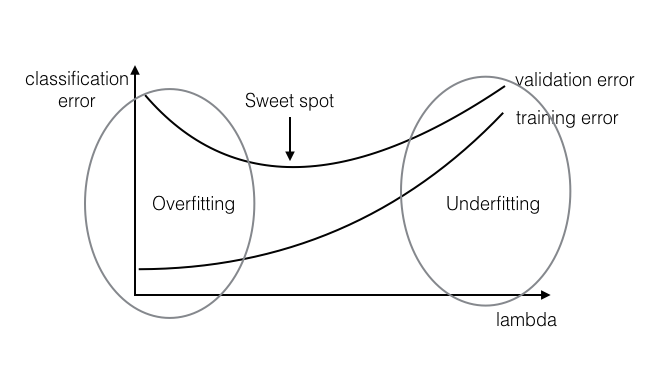
\includegraphics[width=0.7\textwidth]{underoverfit.png}











\newpage
\section{Machine learning 202: Perceptrons and SVM's for classification}
\subsection{Perceptron learning}

\subsection{Hard SVM learning}
The goal in designing the Support Vector Machine is to find the \textbf{maximum separating hyperplane} for our (perfectly separated) binary clusters. To remind you, the figure again (actually, the perpendicular separation between the two clusters is measured from the middle plane, the separation between the two is $2\cdot\text{margin}$, unlike what the figure may suggest):
\begin{center}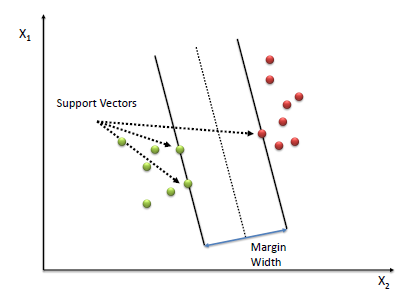
\includegraphics[width=0.5\textwidth]{SVM.png}\end{center}

So we now state that we want to maximize a margin while (for homogeneous coordinates),
\begin{equation}
    y\vec{w}^t\vec{x} \geq m,
\end{equation}
for the cases:
\begin{equation}
    y = \begin{cases} -1 &\vec{w}^T\vec{x}\leq m,\\
                      +1 &\vec{w}^T\vec{x}>m.\end{cases}
\end{equation}

We can measure the margin the following way. Assuming it exists, then there is at least one support vector $\vec{x}^+$ and one support vector $\vec{x}^-$ corresponding to the two clusters. Then we know that we can take their difference $(\vec{x}^+-\vec{x}^-)$ and project it in the unit-vector direction of $\vec{w}$. From the figure we specified that the total separation is $2\cdot\text{margin}$, thus:
\begin{equation}
    2\cdot\text{margin} = \frac{\vec{w}^T}{\abso*{\vec{w}}}(\vec{x}^+-\vec{x}^-)=\frac{2m}{\abso*{\vec{w}}}.
\end{equation}
Note that the margin is thus given by $m/\abso*{\vec{w}}$, we can vary the two parameters inversely proportional and find an infinite number of solutions with the same margin... So, let's choose $m=1$, such that we get the following optimization problem:
\begin{mymathbox}[ams align, title={Hard-margin SVM optimization (primal)}, colframe=blue!30!black, center title]
    \text{Maximize $1/\abso*{\vec{w}}$, i.e., minimize $\abso*{\vec{w}}$:}&\quad \frac{1}{2}\vec{w}^T\vec{w},\\
    \text{Subject to:}&\quad y\vec{w}^T\vec{x}\geq 1.
\end{mymathbox}

\begin{spexample}[Solving SVM with Lagrangian]
    We can convert the SVM problem to a dual problem of the Lagrangian, simply putting the minimization object and constraints in one function, penalizing missing the constraints with factors $\alpha$:
    \begin{equation}
        L(\vec{w},\alpha) = \frac{1}{2}\vec{w}^T\vec{w} - \sum_{n=1}^N\alpha_n \left[y_n\vec{w}^T\vec{x}_n-1\right].\label{eq:lagrangian}
    \end{equation}
    We then set its partial derivatives for $\vec{w}$ to 0:
    \begin{equation}
        \frac{\partial L(\vec{w},\alpha)}{\partial \vec{w}} = \vec{w} - \sum_{n=1}^N \alpha_ny_n\vec{x}_n \equiv 0 \Longleftrightarrow \vec{w} = \sum_{n=1}^N \alpha_ny_n\vec{x}_n.\label{eq:findw}
    \end{equation}
    Substituting into eq. \eqref{eq:lagrangian} provides:
    \begin{equation}
        L(\vec{w},\alpha) = \frac{1}{2}\sum_{i=1}^N\sum_{j=1}^N \alpha_i\alpha_j y_iy_j \vec{x}_i^T\vec{x}_j - \sum_{n=1}^N\sum_{i=1}^N\alpha_n\alpha_i y_ny_i\vec{x}_n^T\vec{x}_i + \sum_{n=1}^N\alpha_n,
    \end{equation}
    which we can simplify to:
    \begin{equation}
        L(\vec{w},\alpha) = \sum_{n=1}^N\alpha_n - \frac{1}{2}\sum_{i=1}^N\sum_{j=1}^N \alpha_i\alpha_j y_iy_j \vec{x}_i^T\vec{x}_j.
    \end{equation}
    This gives rise to the dual problem for SVM:
    \begin{mymathbox}[ams align, title={SVM optimization (dual problem)}, colframe=blue!30!black, center title]
        \text{Minimize:}&\quad L(\vec{w},\alpha)=\sum_{n=1}^N\alpha_n - \frac{1}{2}\sum_{i=1}^N\sum_{j=1}^N \alpha_i\alpha_j y_iy_j \vec{x}_i^T\vec{x}_j,\\
        \text{Subject to:}&\quad \forall_i,\ \alpha_i \geq 0,\\
        &\quad\hphantom{\forall_i,\ }\sum_{n=1}^N\alpha_n y_n = 0,
    \end{mymathbox}
    {\flushleft Where} the final constraint comes out due to the homogenized constraint $(\vec{x})_1=1$ for which we, apparently, don't want to minimize the $L^2$ norm. Thus the actual Lagrangian formulation had to be:
    \begin{equation}
        L(\vec{w},\alpha)=\frac{1}{2}\vec{w}^T\vec{w} - \sum_{n=1}^N \alpha_n \left[ y_n(\vec{w}^T\vec{x} + b) -1 \right].
    \end{equation}
    
    We then, furthermore, know that the $\alpha_i$ values are only required at the support vector locations which will give us the answer to the primal problem (\textbf{Kuhn-Tucker Conditions}), i.e., the coefficients $\alpha_i$ are an incredibly sparse set; and we compute $\vec{w}$ from eq. \eqref{eq:findw}.
    
    The advantageous feature of this formulation is that we have the inner product $\vec{x}^T\vec{x}$, such that a data-transformation $\phi(\vec{x}_i)^T\phi(\vec{x}_j)$ can be replaced by a more efficient transformation $k(\vec{x}_i,\vec{x}_j)$ that computes this inner product for us, thus a non-linear \textbf{kernelized SVM} is easily found:
    \begin{equation}
        L(\vec{w},\alpha) = \sum_{n=1}^N\alpha_n - \frac{1}{2}\sum_{i=1}^N\sum_{j=1}^N \alpha_i\alpha_j y_iy_j k(\vec{x}_i,\vec{x}_j).
    \end{equation}    
\end{spexample}

\subsection{Soft-margin SVM}
Variations on the theme are then easily made. We can allow some `slack' in the classification, such that:
\begin{equation}
    y_i(\vec{w}^T\vec{x}+w_0) \geq m(1-\xi_i),\quad \xi_i\geq 0,
\end{equation}
where of course we want $\xi_i=0$ for most points. In other words, we want to penalize those occurrences of $\xi_i$ as much as possible. A useful parameterization of the problem is found to be:
\begin{mymathbox}[ams align, title={Soft-margin SVM optimization (primal)}, colframe=blue!30!black, center title]
    \text{Minimize $\abso*{\vec{w}}$:}&\quad \frac{1}{2}\vec{w}^T\vec{w} + C\sum_{n=1}^N\xi_n,\\
    \text{Subject to:}&\quad y(\vec{w}^T\vec{x}+w_0)\geq 1-\xi_i,\\
    &\quad \forall_i,\ \xi_i \geq 0.
\end{mymathbox}
{\flushleft The} solution happens to have the same Lagrangian $L$, just different secondary constraints!

\newpage
\section{Lecture 3: Density Estimation in Regression; Parametric Models}
We start with parametric density estimation: we assume a parametric form of the density (e.g., Gaussian, \dots) and estimate the location and width of parameters such as mean and variance. Then we do the maximum likelihood estimation, i.e., for which parameter do we optimally fit the data:
\begin{mymathbox}[ams align, title={Maximum likelihood model parameter}, colframe=blue!30!black, center title]
        \hat{\theta}_{ML} \in \argmax_{\theta} \mathbb{P}(\mathcal{X}^\text{train}|\theta).
\end{mymathbox}
{\flushleft The} method of finding this $\hat{\theta}$ is to consider it to consider $\mathbb{P}(X|\theta)$ a continuous function of $\theta$, for which the maxima has a 0 derivative, which we must simply find:
\begin{mymathbox}[ams align, title={Maximum likelihood procedure}, colframe=blue!30!black, center title]
        \hat{\theta}_{ML} \Rightarrow \nabla_{\theta}\log\left( \mathbb{P}(\mathcal{X}^\text{train}|\hat{\theta}_{ML})\right)=0.
\end{mymathbox}
\begin{testexample}[Mean of Gaussian]
    It is helpful to go through derivations like this one, at least once. The Gaussian for univariate data is $\mathcal{N}(\mu,\sigma)=\frac{1}{\sqrt{2\pi\sigma^2}}e^{-\frac{(x-\mu)^2}{2\sigma^2}}$. The maximum likelihood for $\mu$ based on $N$ samples is the found through:
    \begin{align}
         0 &\equiv \frac{\partial}{\partial \mu}\left( \sum_{i=1}^N\left( -\frac{1}{2}\log( 2\pi\sigma^2 ) - \frac{(x_i-\mu)^2}{2\sigma^2}\right) \right),\\
        & \equiv \frac{\partial}{\partial \mu}\left( \sum_{i=1}^N \left( - \frac{(x_i-\mu)^2}{2\sigma^2} \right)\right), \\
        & \equiv \sum_{i=1}^N\frac{(x_i-\mu)}{\sigma^2} = \left(\sum_{i=1}^N x_i\right)-N\mu \Longleftrightarrow \hat{\mu} =\frac{1}{N}\sum_{i=1}^N x_i.
    \end{align}
    This aligns with our understanding of the expected value based on samples, $\mathbb{E}(x_{i=1,\dots,N})$.
\end{testexample}

\newpage
\subsection{Model selection 1: K-fold cross-validation}
So we establish that there really are two tasks to carry out in machine learning: model fitting and model selection. Leaving the model fitting for later sections, we first focus on model selection methods. The \textbf{K-Fold cross-validation} method uses the hold-out strategy from the previous section, but does so $K$ times, \textit{splitting the data into $K$ non-overlapping portions}. With $N$ samples in the full training data, we then compute $K$ times an intermediate validation score for a chosen model $\hat{f}$:
\begin{equation}
    \hat{R}_k(\hat{f},\mathcal{X}^\text{train}\setminus\mathcal{X}^\text{validate$_k$},\mathcal{Y}^\text{train}\setminus\mathcal{Y}^\text{validate$_k$}) = \frac{1}{(1-\frac{1}{K})N}\sum_{n=1}^{(1-\frac{1}{K})N} \mathbb{I}_{\hat{f}(x_n)\neq y_n}.
\end{equation}
We then sum up all $K$ validation scores to obtain the final error measure:
\begin{equation}
    \hat{R}(\hat{f},\mathcal{X}^\text{train},\mathcal{Y}^\text{train}) = \frac{1}{K}\sum_{k=1}^K \hat{R}_k(\hat{f},\mathcal{X}^\text{train}\setminus\mathcal{X}^\text{validate$_k$},\mathcal{Y}^\text{train}\setminus\mathcal{Y}^\text{validate$_k$})
\end{equation}
For $K=N$ this equals to \textbf{`leave-one out cross-validation' (LOOCV)}, but this can take a long time. However, it is unbiased. In practice, $K\in[5,10]$ is a typical choice.

\begin{figure}[!h]
    \centering
    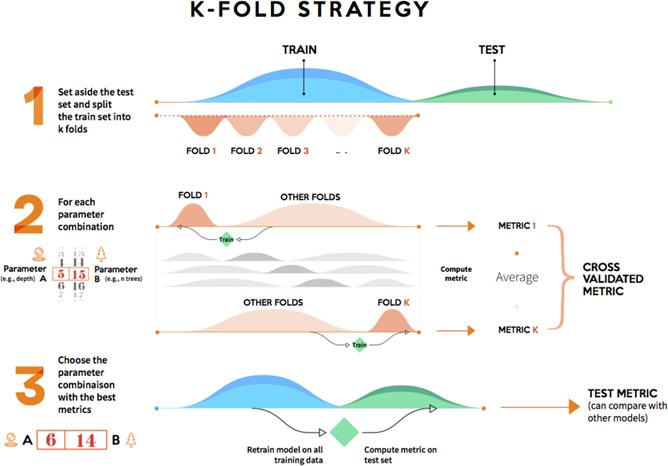
\includegraphics[width=0.8\textwidth]{kfold-strategy.jpg}
    \caption{A graphical example of $K$-fold cross-validation. The training set is split into $K$ \textit{folds}; then for each model-parameter combination the model is trained in the $K-1$ sets and scored on the $K$ remaining fold. The average score is used as the cross-validated metric. The optimal model-parameter combination can then be used to train the final model.}
    \label{fig:my_label}
\end{figure}

\subsection{Bootstrap}
.632 bootstrap
\subsection{Jack-knife}

\section{Regression}


\subsection{Regression}
\subsubsection{The setting}
We, abstractly, consider an object space $\mathcal{O}$ with data-space for $d$-dimensional data leading to a single output, sorted in tuples: $\mathcal{Z}=\{(x_i,y_i)\in\mathbb{R}^d\times\mathbb{R}:i\leq i \leq n\}$. We use a model with output $Y$ and input $X=(X_0,X_1,\dots,X_d)$ features with $X_0=1$\footnote{For linear regression we assume $y=\mathbf{a}^T \mathbf{x}+b$, which we could also write as $y=\mathbf{a}^T\mathbf{x}$ when $x_0=1$ and $a_0=b$.} and $\epsilon$ the noise with expected value $\mathbb{E}[\epsilon]=0$:
\begin{equation}
    \mathbf{Y}=f(\mathbf{X},\theta)+\epsilon.
\end{equation}
In the \textbf{Bayesian} view, $\mathbf{X}$, $\mathbf{Y}$ and $\theta$ are random variables, which brings with it useful properties I think. In the view of \textbf{parametric statistics}, the form of $\mathbb{P}(\mathbf{X},\mathbf{Y}|\theta)$ is given, we want to estimate $\theta$ for the likelihood $\mathbb{P}(\mathbf{Y}|\mathbf{X})$. In \textbf{non-parametric statistics} we sample $\mathbf{X}$ and $\mathbf{Y}$ to estimate the likelihood $\mathbb{P}(X,Y)$. In \textbf{statistical learning theory} we directly minimize the empirical risk function ($\arg\min_{f\in\mathcal{C}}\hat{R}(f,\mathcal{Z}^\text{train})$) without estimating the likelihood.

\subsubsection{The frequentist vs Bayesian view}
Bayes' rule (preferred by the teacher over Bayes' theorem):
\begin{equation}
    \mathbb{P}(\text{model}|\text{data})=\frac{\mathbb{P}(\text{data}|\text{model})\mathbb{P}( \text{model} )  }{ \mathbb{P}(\text{data})   } = \text{posterior}=\frac{\text{likelihood}\cdot\text{prior}}{\text{evidence}}.
\end{equation}
This is in contrast with Frequentism. However, these guys did come up with the \textbf{maximum likelihood} method, Fisher information, sampling theory and hypothesis testing.

\subsubsection{Ex: Regression with maximum likelihood}
This is extra, from Bishop's `Pattern Recognition \& Machine Learning'. We will work systematically in the below.
\begin{enumerate}
    \item \textbf{The model}. We assume that we can write the model as a polynomial function:
    \begin{equation}
        y(x,\mathbf{w}) = w_0+w_1x+w_2x^2+\dots+w_Mx^M=\sum_{j=0}^M w_jx^j.
    \end{equation}
    \item \textbf{One data distribution}. We assume that we can write the one data-point $t$ given an $x$, using a normal distribution with inverse variance $\beta^{-1}$ (giving the precision) and a mean given by the equation for $y$ above:
    \begin{equation}
        \mathbb{P}(t|x,\mathbf{w},\beta) = \mathcal{N}(t|y(x,\mathbf{w}),\beta^{-1}).
    \end{equation}
    \item \textbf{The likelihood function}. We can now write down the likelihood of the data given the model. Assuming that the data was drawn iid we simply get the product of the individual probability distributions:
    \begin{equation}
        \mathbb{P}(\mathbf{t}|\mathbf{x},\mathbf{w},\beta) = \prod_{n=1}^N \mathcal{N}(t_n|y(x_n,\mathbf{w}),\beta^{-1}).
    \end{equation}
    \item \textbf{The log likelihood function}. Taking the logarithm of the function above:
    \begin{align}
        \log \mathbb{P}(\mathbf{t}|\mathbf{x},\mathbf{w},\beta) & = \log \prod_{n=1}^N \mathcal{N}(t_n|y(x_n,\mathbf{w}),\beta^{-1}),\\
        & = \sum_{n=1}^N\log\left(\mathcal{N}(t_n|y(x_n,\mathbf{w}),\beta^{-1})\right),\\
        &=\sum_{n=1}^N\log\left( \frac{\sqrt{\beta}}{\sqrt{2\pi}} e^{-\frac{\beta}{2}(t_n-y(x_n,\mathbf{w}))^2 }         \right), \\
        &=\sum_{n=1}^N\left[\log\left( \sqrt{\beta} \right) - \log \left(\sqrt{2\pi} \right) + \log \left( e^{-\frac{\beta}{2}(t_n-y(x_n,\mathbf{w}))^2 }         \right)\right],\\
        &=\sum_{n=1}^N\left[\frac{1}{2}\log\left(\beta\right) - \frac{1}{2}\log \left(2\pi\right) + \left( -\frac{\beta}{2}(t_n-y(x_n,\mathbf{w}))^2          \right)\right],\\
        &=\frac{N}{2}\bigg(\log(\beta) - \log(2\pi)\bigg) + \sum_{n=1}^N \left( -\frac{\beta}{2}(t_n-y(x_n,\mathbf{w}))^2          \right)
    \end{align}
    \item \textbf{The maximum log-likelihood}. Taking the derivative w.r.t. $\mathbf{w}$, and setting this to zero, should give the optimal model:
    \begin{align}
        \frac{\partial \log\mathbb{P}(\mathbf{t}|\mathbf{x},\mathbf{w},\beta)}{\partial \mathbf{w}} &= - \frac{\beta}{2}\sum_{n=1}^N(t_n-y(x_n,\mathbf{w}))^2,\\
        &=-\frac{\beta}{2}\sum_{n=1}^N\sum_{j=1}^M(t_n-w_jx_n^j)^2,\\
        &=0\Longleftrightarrow \text{least-squares solution }\mathbf{w}_\text{ML}. 
    \end{align}
    Similarly, we can derive the optimal precision (inverse standard-deviation) of the likelihood function, $\beta_\text{ML}$:
    \begin{align}
        \frac{\partial \log\mathbb{P}(\mathbf{t}|\mathbf{x},\mathbf{w},\beta)}{\partial \beta} & = \frac{N}{2\beta} - \sum_{n=1}^N\left( \frac{1}{2}(t_n - y(x_n,\mathbf{w}_\text{ML}))^2 \right),\\
        &=0 \Longleftrightarrow \frac{1}{\beta_\text{ML}} = \frac{1}{N}\sum_{n=1}^N(t_n - y(x_n,\mathbf{w}_\text{ML}))^2.
    \end{align}
    \item \textbf{Predict new data}. We can no make predictions for new values of $x$, in terms of the predictive distribution rather than a point-estimate that we usually get:
    \begin{equation}
        \mathbb{P}(t|x,\mathbf{w}_\text{ML},\beta_\text{ML}) = \mathcal{N}(t|y(x,\mathbf{W}_\text{ML}),\beta_{\text{ML}}^{-1}).
    \end{equation}
    \item \textbf{Introducing a prior for $\mathbf{w}$}. If we assume that the coefficients $\mathbf{w}$ are spread with a Gaussian distribution:
    \begin{equation}
        \mathbb{P}(\mathbf{w}|\alpha) = \mathcal{N}(\mathbf{w}|0,\alpha^{-1})
    \end{equation}
    We can now make a comment about the \textit{posterior} distribution! Indeed, we know that:
    \begin{equation}
        \mathbb{P}(\mathbf{w}|\mathbf{x},\mathbf{t},\alpha,\beta) \propto \mathbb{P}(\mathbf{t}|\mathbf{x},\mathbf{w},\beta)\mathbb{P}(\mathbf{w}|\alpha).
    \end{equation}
    Taking the logarithm of the RHS of the equation we find:
    \begin{align}
        \log\left( \mathbb{P}(\mathbf{t}|\mathbf{x},\mathbf{w},\beta)\mathbb{P}(\mathbf{w}|\alpha) \right) &=  \\
        \frac{N}{2}\bigg(\log(\beta) - \log(2\pi)\bigg) + \sum_{n=1}^N \left( -\frac{\beta}{2}(t_n-y(x_n,\mathbf{w}))^2          \right)& + \frac{M+1}{2}\log\left( \frac{\alpha}{2\pi} \right) - \frac{\alpha}{2}\mathbf{w}^T\mathbf{w}.
    \end{align}
    The extremum is then found through the derivative to $\mathbf{w}$:
    \begin{align}
        \frac{\partial -\log\left( \mathbb{P}(\mathbf{t}|\mathbf{x},\mathbf{w},\beta)\mathbb{P}(\mathbf{w}|\alpha) \right)}{\partial \mathbf{w}} &=  \sum_{n=1}^N \left( \frac{\beta}{2}(t_n-y(x_n,\mathbf{w}))^2          \right) + \frac{\alpha}{2}\mathbf{w}^T\mathbf{w}, \\
        &=0\Longleftrightarrow \text{the ridge-regression solution with }\lambda=2\frac{\alpha}{\beta}.
    \end{align}
    \item \textbf{Predicting values given the posterior distribution}. We can `simply' marginalize the known quantities now to introduce new $t^*$ for $x^*$:
    \begin{equation}
        \mathbb{P}(t^*|x^*,\mathbf{x},\mathbf{t}) = \int \mathbb{P}(t^*|x^*,\mathbf{w})\mathbb{P}(\mathbf{w}|\mathbf{x},\mathbf{t}) \di \mathbf{w}
    \end{equation}
    The solution to this problem is a normal distribution itself with a mean and variance. The solution to this can be found with matrix calculus. Basically, the mean is our usual solution to the problem, and the variance is the information gained: an uncertainty boundary (or $\pm1$ standard deviation boundary around the mean).
\end{enumerate}
\begin{figure}
    \centering
    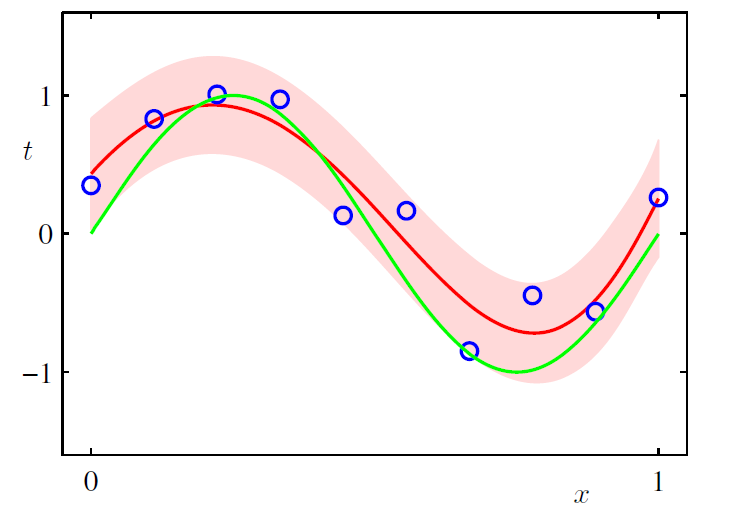
\includegraphics[width=0.5\textwidth]{bishop.png}
    \caption{A Bayesian version of regression with mean (red) and $\pm1$ standard deviation (shaded), given a limited number of data-points, and some expectations about the noise levels.}
    \label{fig:bayesregr}
\end{figure}



\end{document}